% Figuras y tablas M1 (notebook 01_diagnostico_operacional.ipynb) — incluido desde presentacion_demo.tex
% Rutas relativas al directorio demo_caso_tecnico/

\subsection{Panel: números descriptivos}

\begin{frame}{Resumen numérico — \texttt{describe}}
  \centering
  \renewcommand{\arraystretch}{1.35}
  {\normalsize
  \begin{tabular}{@{}lrrrr@{}}
    \toprule
    & \texttt{HOUR} & \texttt{ratio} & \texttt{PRECIPITATION\_MM} & \texttt{EARNINGS} \\
    \midrule
    count & 10080{,}0000 & 10080{,}0000 & 10080{,}0000 & 10080{,}0000 \\
    mean  & 11{,}5000 & 0{,}8179 & 0{,}2467 & 57{,}6961 \\
    std   & 6{,}9225 & 0{,}5509 & 1{,}2650 & 8{,}2928 \\
    min   & 0{,}0000 & 0{,}0000 & 0{,}0000 & 49{,}0000 \\
    25\%  & 5{,}7500 & 0{,}5000 & 0{,}0000 & 52{,}4000 \\
    50\%  & 11{,}5000 & 0{,}8000 & 0{,}0000 & 55{,}6000 \\
    75\%  & 17{,}2500 & 1{,}0968 & 0{,}0000 & 58{,}7000 \\
    max   & 23{,}0000 & 5{,}6667 & 10{,}3000 & 97{,}0000 \\
    \bottomrule
  \end{tabular}
  }

  \vspace{0.55em}
  \footnotesize
  \textbf{Nota:} si \texttt{CONNECTED\_RT}${}=0$, \texttt{ratio} es NaN y no cuenta en \texttt{describe}; en este panel las cuatro columnas muestran \texttt{count}${}=10\,080$.
\end{frame}

\begin{frame}{Cobertura del panel}
  \centering
  \renewcommand{\arraystretch}{1.35}
  {\normalsize
  \begin{tabular}{@{}lr@{}}
    \toprule
    \textbf{Métrica} & \textbf{Valor} \\
    \midrule
    Filas totales (observaciones en el extracto) & 10\,080 \\
    Zonas distintas (\texttt{ZONE}) & 14 \\
    Horas distintas (\texttt{HOUR}) & 24 \\
    Sin clasificación operativa (\texttt{ratio} NaN, sin etiqueta) & 0 \\
    \bottomrule
  \end{tabular}
  }

  \vspace{0.75em}
  {\normalsize
  Estructura nominal del caso: \textbf{30 días $\times$ 24 h $\times$ 14 zonas} $= 10\,080$ celdas, alineado con el Excel de referencia.
  }
\end{frame}

\begin{frame}{Clasificación operativa — conteos y \% (sobre filas con etiqueta)}
  \begingroup
  \centering
  \renewcommand{\arraystretch}{1.35}
  {\normalsize
  \begin{tabular}{@{}lrrp{0.52\textwidth}@{}}
    \toprule
    \textbf{\texttt{clasificacion}} & \textbf{$n$ filas} & \textbf{\%} & \textbf{Criterio sobre \texttt{ratio}} \\
    \midrule
    intermedio   & 4807 & 47{,}69 & Resto: $[\,0{,}5,\,0{,}9)$ o $(\,1{,}2,\,1{,}8\,]$. \\
    saludable    & 2503 & 24{,}83 & $0{,}9 \le \texttt{ratio} \le 1{,}2$. \\
    sobre\_oferta & 2257 & 22{,}39 & $\texttt{ratio} < 0{,}5$. \\
    saturacion   & 513  & 5{,}09  & $\texttt{ratio} > 1{,}8$. \\
    \bottomrule
  \end{tabular}
  }
  \par
  \endgroup

  \begin{piegraficafoot}
  La columna \texttt{clasificacion} resume el estado frente a umbrales de \texttt{ratio} del diagnóstico (saludable, saturación, etc.). Los porcentajes son sobre filas con categoría (aquí, las 10\,080 con \texttt{ratio} válido).
  \end{piegraficafoot}

  \begin{piegrafica}
  La mayoría del panel está fuera de saturación; $\approx 5\%$ de celdas superan el umbral operativo. IC95\% Wilson para la proporción global en saturación: $[0{,}0468,\,0{,}0554]$.
  \end{piegrafica}
\end{frame}

\subsection{Saturación por hora y por zona (P1)}

\begin{frame}{P1 — Saturación por hora del día}
  \begingroup
  \centering
  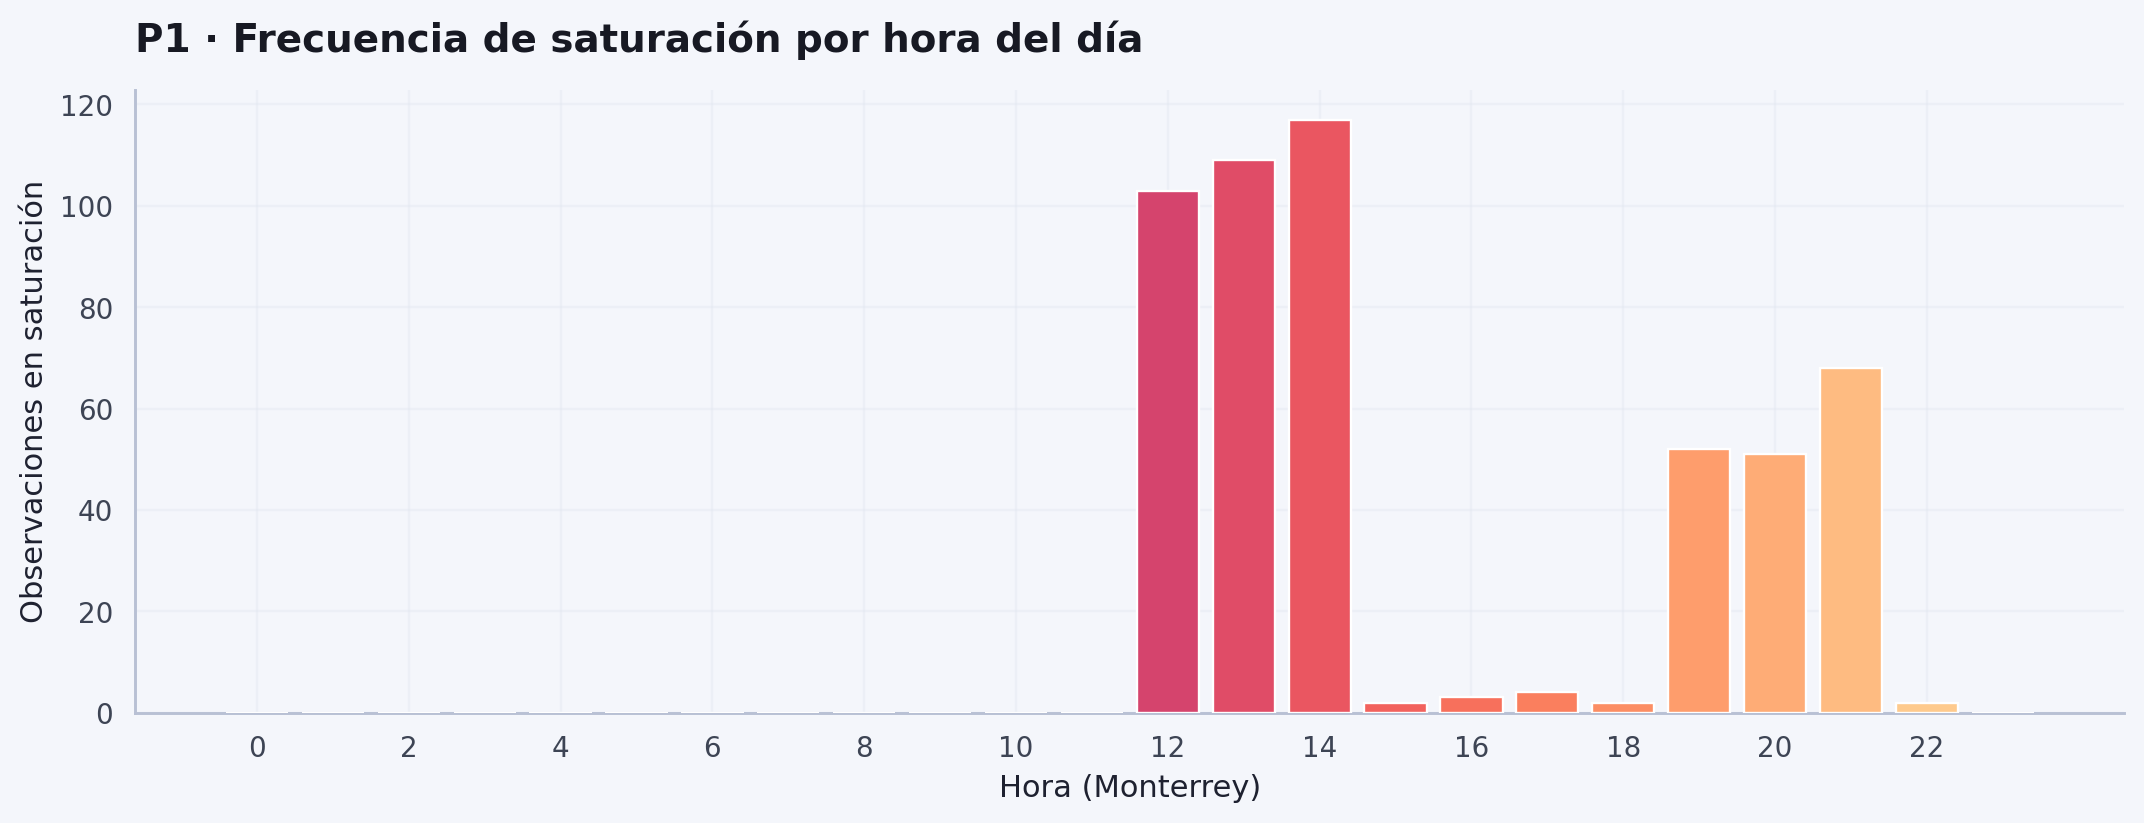
\includegraphics[width=\linewidth,height=0.70\textheight,keepaspectratio]{../modulo1_diagnostico/figures/p1_horas_saturacion.png}
  \par
  \endgroup
  \begin{piegrafica}
  P1 responde \emph{¿a qué horas} aparece más a menudo el ratio por encima del umbral de saturación? No es predicción; es \textbf{conteo} en el historial del Excel.

  El gráfico acumula filas con \texttt{clasificacion}${}=$\texttt{saturacion} (\texttt{ratio}${}>1{,}8$) por hora.
  \end{piegrafica}
\end{frame}

\begin{frame}{P1 — Horas con mayor fracción empírica de saturación}
  \begingroup
  \centering
  \footnotesize
  \renewcommand{\arraystretch}{1.15}
  \begin{tabular}{@{}crr@{}}
    \toprule
    \texttt{HOUR} & $p_{\text{sat}}$ & $n$ \\
    \midrule
    14 & $0{,}2786$ & 420 \\
    13 & $0{,}2595$ & 420 \\
    12 & $0{,}2452$ & 420 \\
    21 & $0{,}1619$ & 420 \\
    19 & $0{,}1238$ & 420 \\
    20 & $0{,}1214$ & 420 \\
    17 & $0{,}0095$ & 420 \\
    16 & $0{,}0071$ & 420 \\
    \bottomrule
  \end{tabular}
  \par
  \endgroup
  \begin{piegraficafoot}
  Salida del notebook (bloque 3c): fracción de filas en saturación por hora, ordenadas; $n=420$ celdas por hora en el panel balanceado.
  \end{piegraficafoot}
\end{frame}

\begin{frame}{P1 — Zonas con más celdas en saturación}
  \begingroup
  \centering
  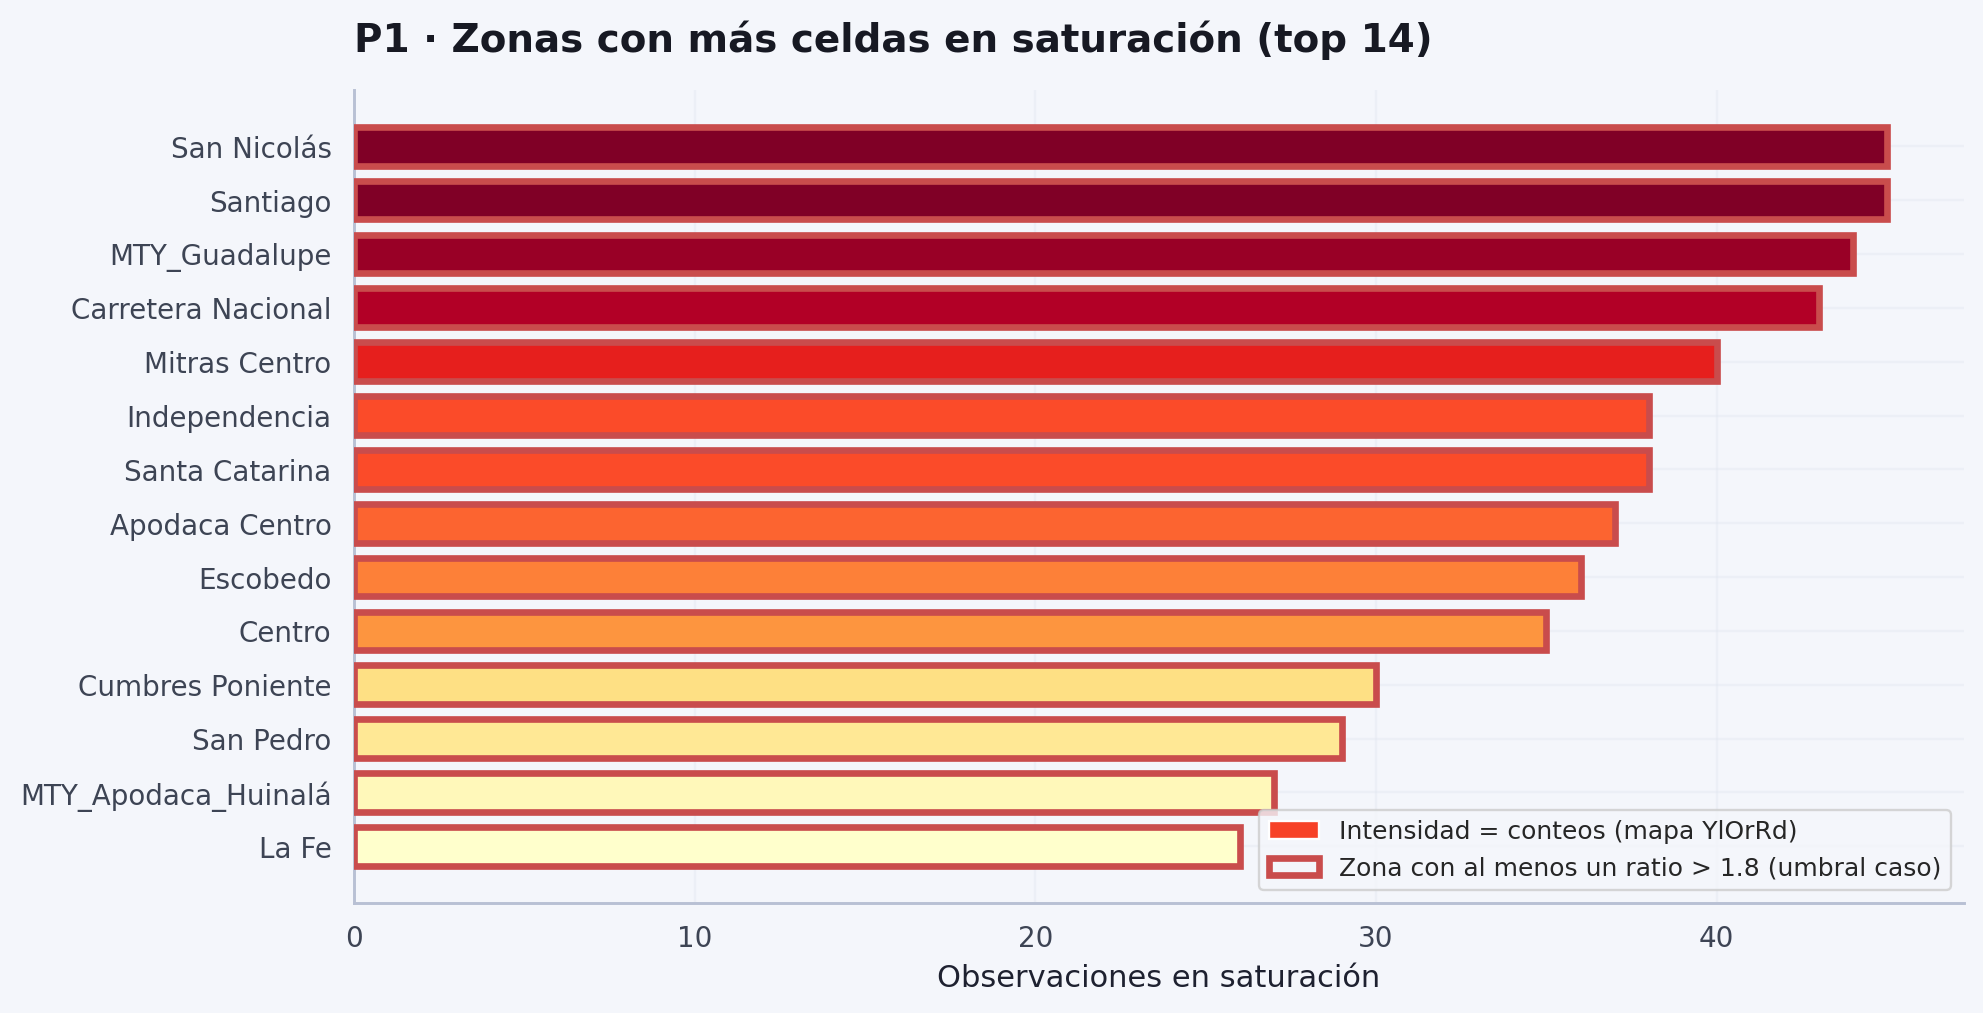
\includegraphics[width=\linewidth,height=0.70\textheight,keepaspectratio]{../modulo1_diagnostico/figures/p1_zonas_saturacion.png}
  \par
  \endgroup
  \begin{piegrafica}
  Ordena territorios por \textbf{frecuencia histórica} de saturación en el mes. Sirve para priorizar dónde mirar primero; no sustituye criterio de zona en vivo.
  \end{piegrafica}
\end{frame}

\subsection{Precipitación: correlación, MCO y diagnósticos (P2)}

\begin{frame}[t]{P2 — Correlaciones Pearson y MCO}
  \begingroup
  \footnotesize
  \centering
  \textbf{Matriz de correlación de Pearson}\\[0.35em]
  \resizebox{0.92\linewidth}{!}{%
  \begin{tabular}{@{}lrrr@{}}
    \toprule
    & \texttt{PRECIPITATION\_MM} & \texttt{ratio} & \texttt{EARNINGS} \\
    \midrule
    \texttt{PRECIPITATION\_MM} & 1{,}000000 & 0{,}318902 & 0{,}226029 \\
    \texttt{ratio}             & 0{,}318902 & 1{,}000000 & 0{,}099885 \\
    \texttt{EARNINGS}          & 0{,}226029 & 0{,}099885 & 1{,}000000 \\
    \bottomrule
  \end{tabular}%
  }
  \par
  \endgroup

  \vspace{0.3em}
  \begingroup
  \footnotesize
  \raggedright
  \noindent
  \textbf{Modelo:} \texttt{ratio} $\sim$ \texttt{PRECIPITATION\_MM} + \texttt{C(HOUR)} + \texttt{C(ZONE)} + \texttt{C(dow)}\\[0.2em]
  Coef.\ \texttt{PRECIPITATION\_MM}: $0{,}080244$ \quad p-valor (MCO clásico): $\approx 2{,}1\times 10^{-231}$\\[0.1em]
  IC95\% coef.\ precipitación: $[0{,}075527,\,0{,}084960]$ \quad $R^2 = 0{,}7180$ \quad $n = 10\,080$\\[0.25em]
  $P(\text{saturación} \mid \text{precip} > 0{,}5) = 0{,}3082$ \quad
  $P(\text{saturación} \mid \text{precip} \le 0{,}5) = 0{,}0377$\\[0.25em]
  \textbf{MCO con SE cluster (zona):} $\beta_{\text{precip}} = 0{,}080244$ \quad SE${}= 0{,}010357$ \quad $p = 9{,}37\times 10^{-15}$ \quad IC95\%: $[0{,}059944,\,0{,}100544]$
  \par
  \endgroup

  \begin{piegrafica}
  Primero la \textbf{correlación de Pearson} (asociación lineal simple). Luego el \textbf{MCO} con controles: el coeficiente de lluvia es \textbf{marginal condicionado} a hora, zona y día.

  Eso reduce confusión por patrones semanales, pero \textbf{no} prueba causalidad por sí solo.
  \end{piegrafica}
\end{frame}

\begin{frame}{P2 — Resumen numérico del ajuste OLS}
  \begingroup
  \footnotesize
  \centering
  \renewcommand{\arraystretch}{1.2}
  \begin{tabular}{@{}lr@{}}
    \toprule
    \textbf{Métrica} & \textbf{Valor} \\
    \midrule
    Modelo & OLS \\
    Variable dependiente & \texttt{ratio} \\
    $R^2$ & 0{,}718 \\
    $R^2$ ajustado & 0{,}717 \\
    Observaciones & 10\,080 \\
    Grados de libertad (modelo / residuos) & 43 / 10\,036 \\
    Estadístico $F$ & 594{,}1 \\
    $\Pr(>F)$ & $\approx 0$ \\
    AIC & 3916{,}2816 \\
    BIC & 4233{,}8871 \\
    Log-verosimilitud & $-1914{,}1$ \\
    Escala (\texttt{Scale}) & 0{,}085974 \\
    \bottomrule
  \end{tabular}
  \par
  \endgroup

  \begin{piegrafica}
  Resumen del ajuste global del MCO principal: $F$ muy grande y $R^2$ alto indican que hora, zona, día y lluvia explican buena parte de la variación del \texttt{ratio} en este panel.

  Es una lectura descriptiva del modelo, no inferencia causal.
  \end{piegrafica}
\end{frame}

\begin{frame}{P2 — Diagnóstico MCO (1/4) — Residuos vs ajustados}
  \begingroup
  \centering
  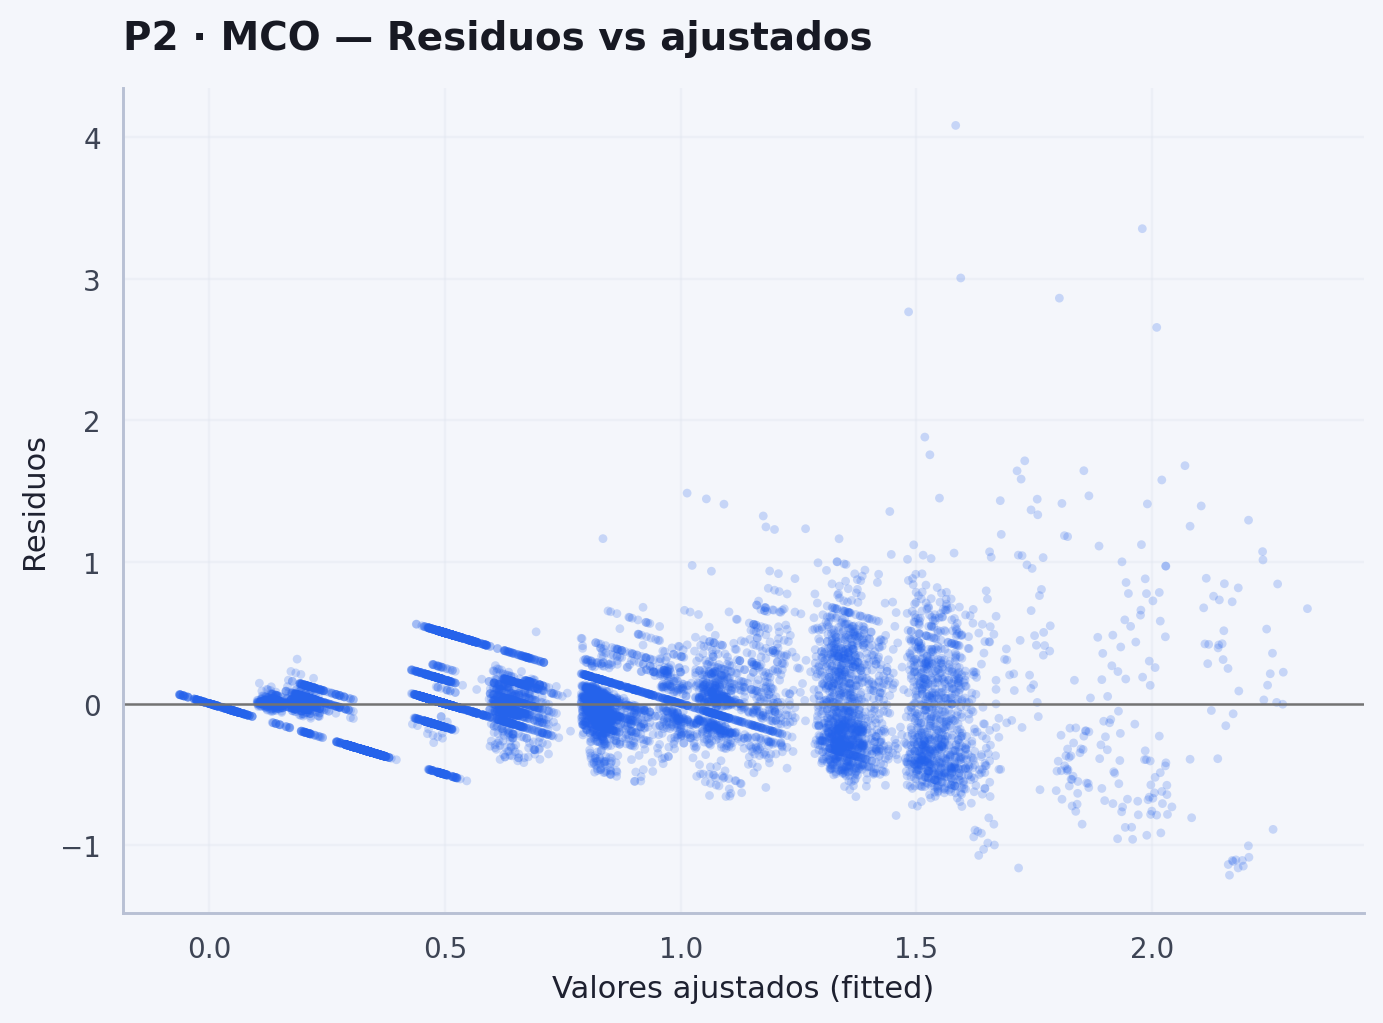
\includegraphics[width=\linewidth,height=0.70\textheight,keepaspectratio]{../modulo1_diagnostico/figures/p2_ols_diagnostico_separados/p2_ols_residuals_vs_fitted.png}
  \par
  \endgroup
  \begin{piegrafica}
  Busca patrones sistemáticos (curvas, abanicos). Si el modelo captura bien la media condicional, la nube debería verse razonablemente aleatoria alrededor de cero.
  \end{piegrafica}
\end{frame}

\begin{frame}{P2 — Diagnóstico MCO (2/4) — QQ de residuos}
  \begingroup
  \centering
  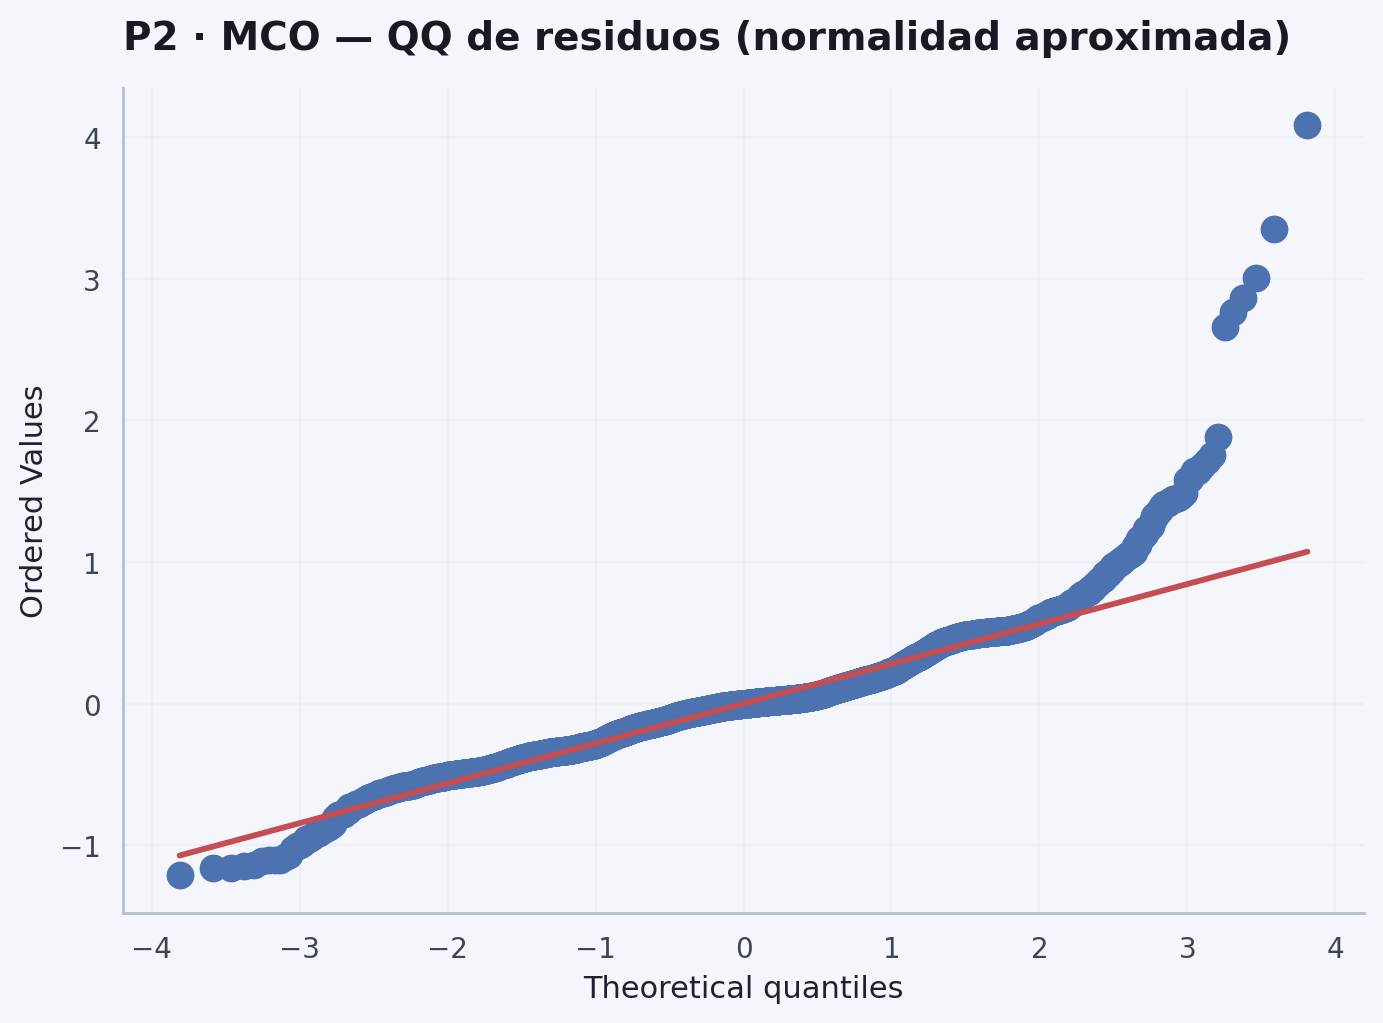
\includegraphics[width=\linewidth,height=0.70\textheight,keepaspectratio]{../modulo1_diagnostico/figures/p2_ols_diagnostico_separados/p2_ols_qq_residuals.png}
  \par
  \endgroup
  \begin{piegrafica}
  Compara la cola de los residuos con la normal. Desviaciones fuertes sugieren colas pesadas o valores atípicos que el modelo lineal no absorbe bien.
  \end{piegrafica}
\end{frame}

\begin{frame}{P2 — Diagnóstico MCO (3/4) — Regresión parcial (lluvia)}
  \begingroup
  \centering
  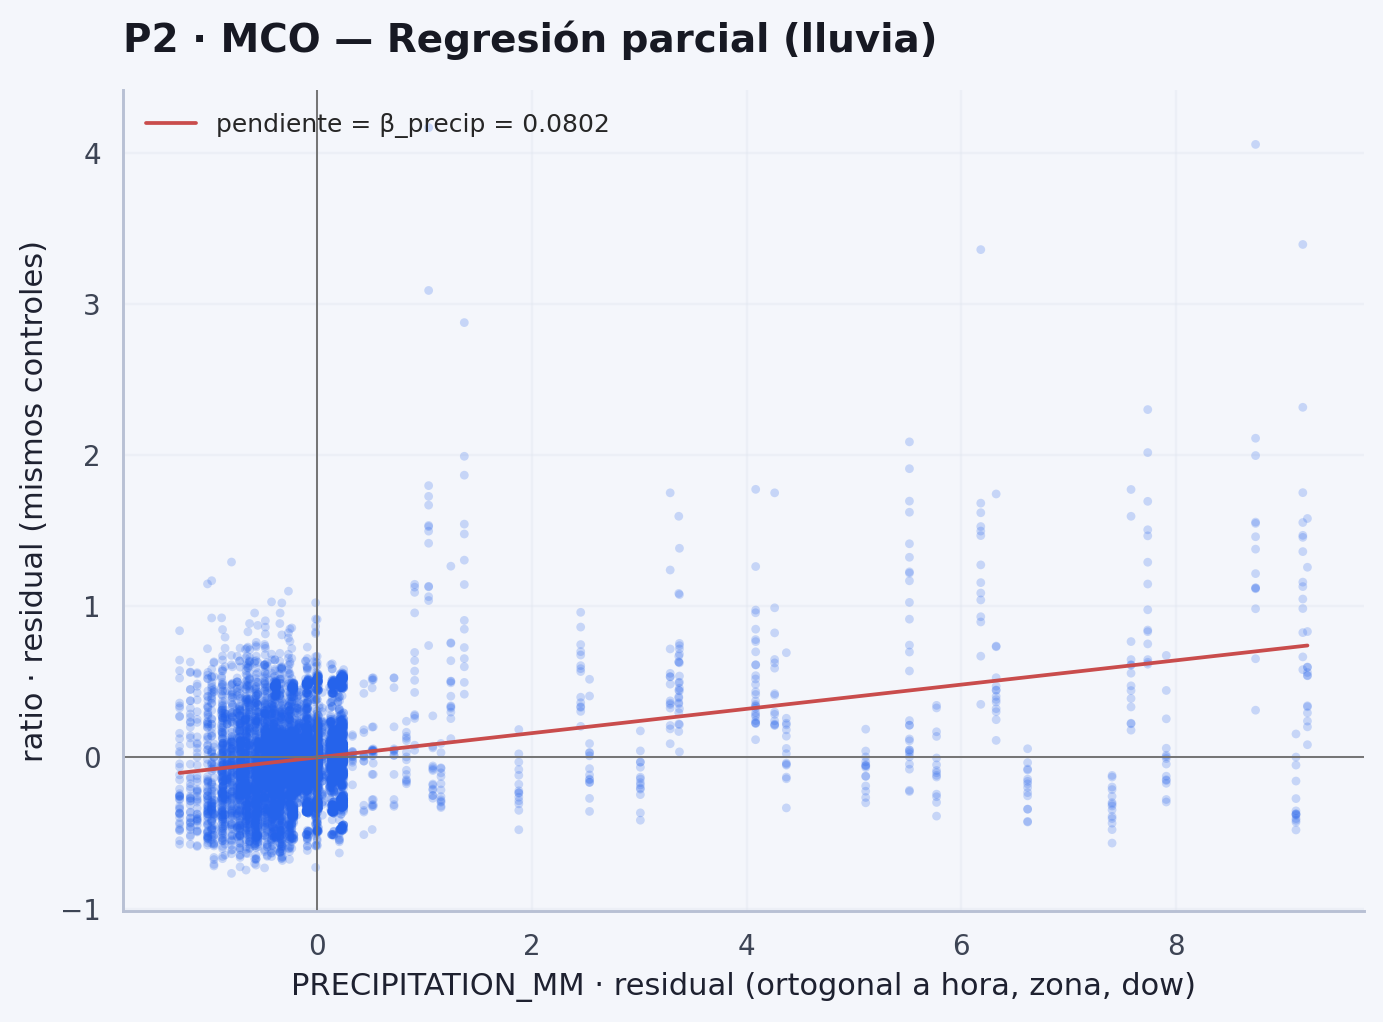
\includegraphics[width=\linewidth,height=0.70\textheight,keepaspectratio]{../modulo1_diagnostico/figures/p2_ols_diagnostico_separados/p2_ols_partial_precip.png}
  \par
  \endgroup
  \begin{piegrafica}
  Relación entre lluvia y ratio \emph{después} de quitar hora, zona y día de la semana: idea de ``pendiente neta'' de precipitación.
  \end{piegrafica}
\end{frame}

\begin{frame}{P2 — Diagnóstico MCO (4/4) — Observado vs ajustado}
  \begingroup
  \centering
  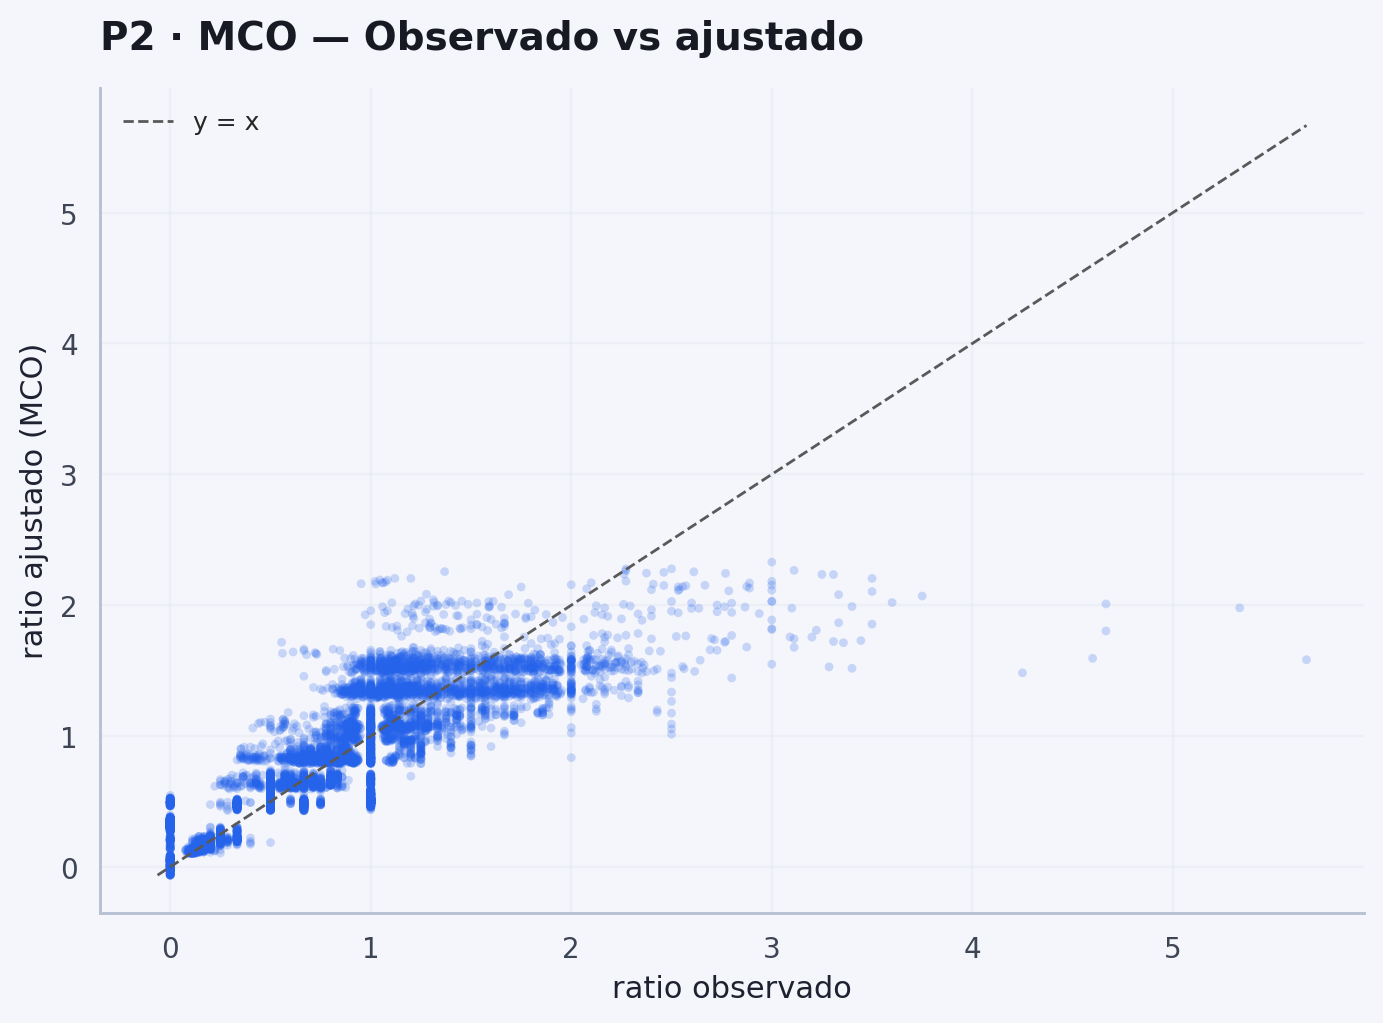
\includegraphics[width=\linewidth,height=0.70\textheight,keepaspectratio]{../modulo1_diagnostico/figures/p2_ols_diagnostico_separados/p2_ols_observed_vs_fitted.png}
  \par
  \endgroup
  \begin{piegrafica}
  Mide qué tan bien el ajuste reproduce el nivel de \texttt{ratio}. Los puntos muy alejados de la diagonal indican celdas mal explicadas por el modelo.
  \end{piegrafica}
\end{frame}

\begin{frame}{P2 — Lluvia, demanda e interacción (lectura cualitativa)}
  \begingroup
  \centering
  \normalsize
  \renewcommand{\arraystretch}{1.35}
  \begin{tabular}{@{}ll@{}}
    \toprule
    \textbf{Hora} & \textbf{Efecto de lluvia} \\
    \midrule
    Mañana & Bajo impacto \\
    Comida & Medio \\
    Cena & \textcolor{rappiaccent}{\textbf{Muy alto}} \\
    \bottomrule
  \end{tabular}
  \par
  \endgroup

  \begin{piegraficafoot}
  La lluvia se asocia a más saturación \textbf{controlando} por hora y zona, pero el efecto \textbf{no es homogéneo}: se \textbf{intensifica en horas de alta demanda} (interacción operativa--externa).

  La tabla es cualitativa y está alineada con GAP~1 (pendiente marginal por hora).
  \end{piegraficafoot}
\end{frame}

\subsection{Exploración, GAP1 y tramos de \texttt{ratio} (P2b)}

\begin{frame}{Exploración — distribución del \texttt{ratio} por zona}
  \begingroup
  \centering
  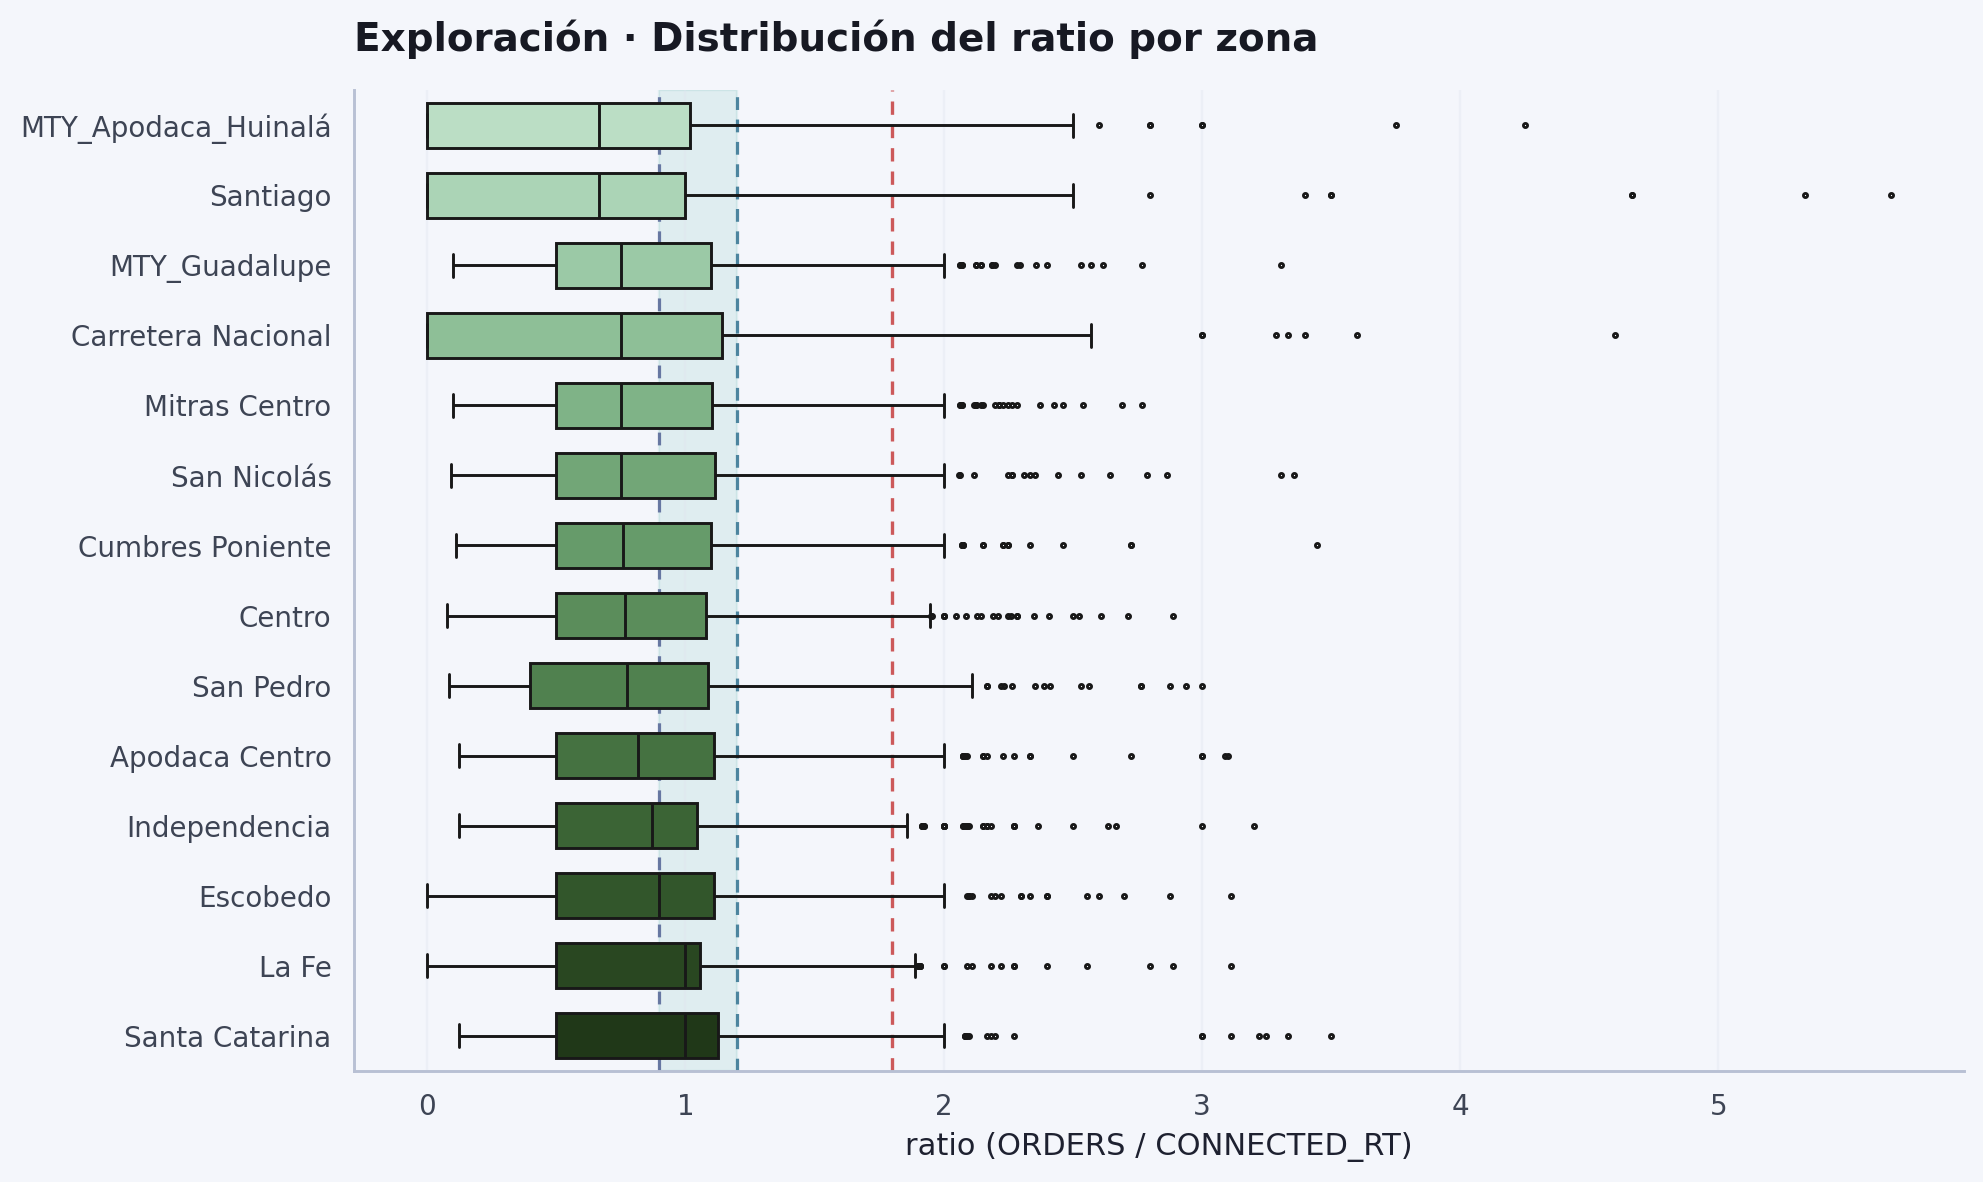
\includegraphics[width=\linewidth,height=0.70\textheight,keepaspectratio]{../modulo1_diagnostico/figures/exploracion_ratio_por_zona.png}
  \par
  \endgroup
  \begin{piegrafica}
  Panorama antes de profundizar: cómo se distribuye el \texttt{ratio} y cómo se compara \textbf{entre zonas} (mediana, dispersión, colas).
  \end{piegrafica}
\end{frame}

\begin{frame}{GAP 1 — Contraste ANOVA (lluvia $\times$ hora)}
  \begingroup
  \footnotesize
  \centering
  \renewcommand{\arraystretch}{1.2}
  \begin{tabular}{@{}lrr@{}}
    \toprule
    \textbf{Modelo} & $R^2$ & $R^2$ adj. \\
    \midrule
    Aditivo (\texttt{precip} + hora + zona + \texttt{dow}) & $0{,}7180$ & $0{,}7168$ \\
    Con interacción \texttt{precip}$\times$\texttt{HOUR} & $0{,}7288$ & $0{,}7271$ \\
    \bottomrule
  \end{tabular}

  \vspace{0.4em}
  \textbf{Contraste de modelos anidados} (mismas $n=10\,080$): $F \approx 23{,}47$, $\Pr(>F) \approx 1{,}1\times 10^{-72}$.
  \par
  \endgroup

  \begin{piegrafica}
  La interacción lluvia$\times$hora mejora el ajuste de forma \textbf{estadísticamente muy fuerte}: el efecto de la lluvia sobre el \texttt{ratio} \emph{cambia} según la hora (heterogeneidad horaria).
  \end{piegrafica}
\end{frame}

\begin{frame}{GAP 1 — Pendiente marginal de precipitación por hora}
  \begingroup
  \centering
  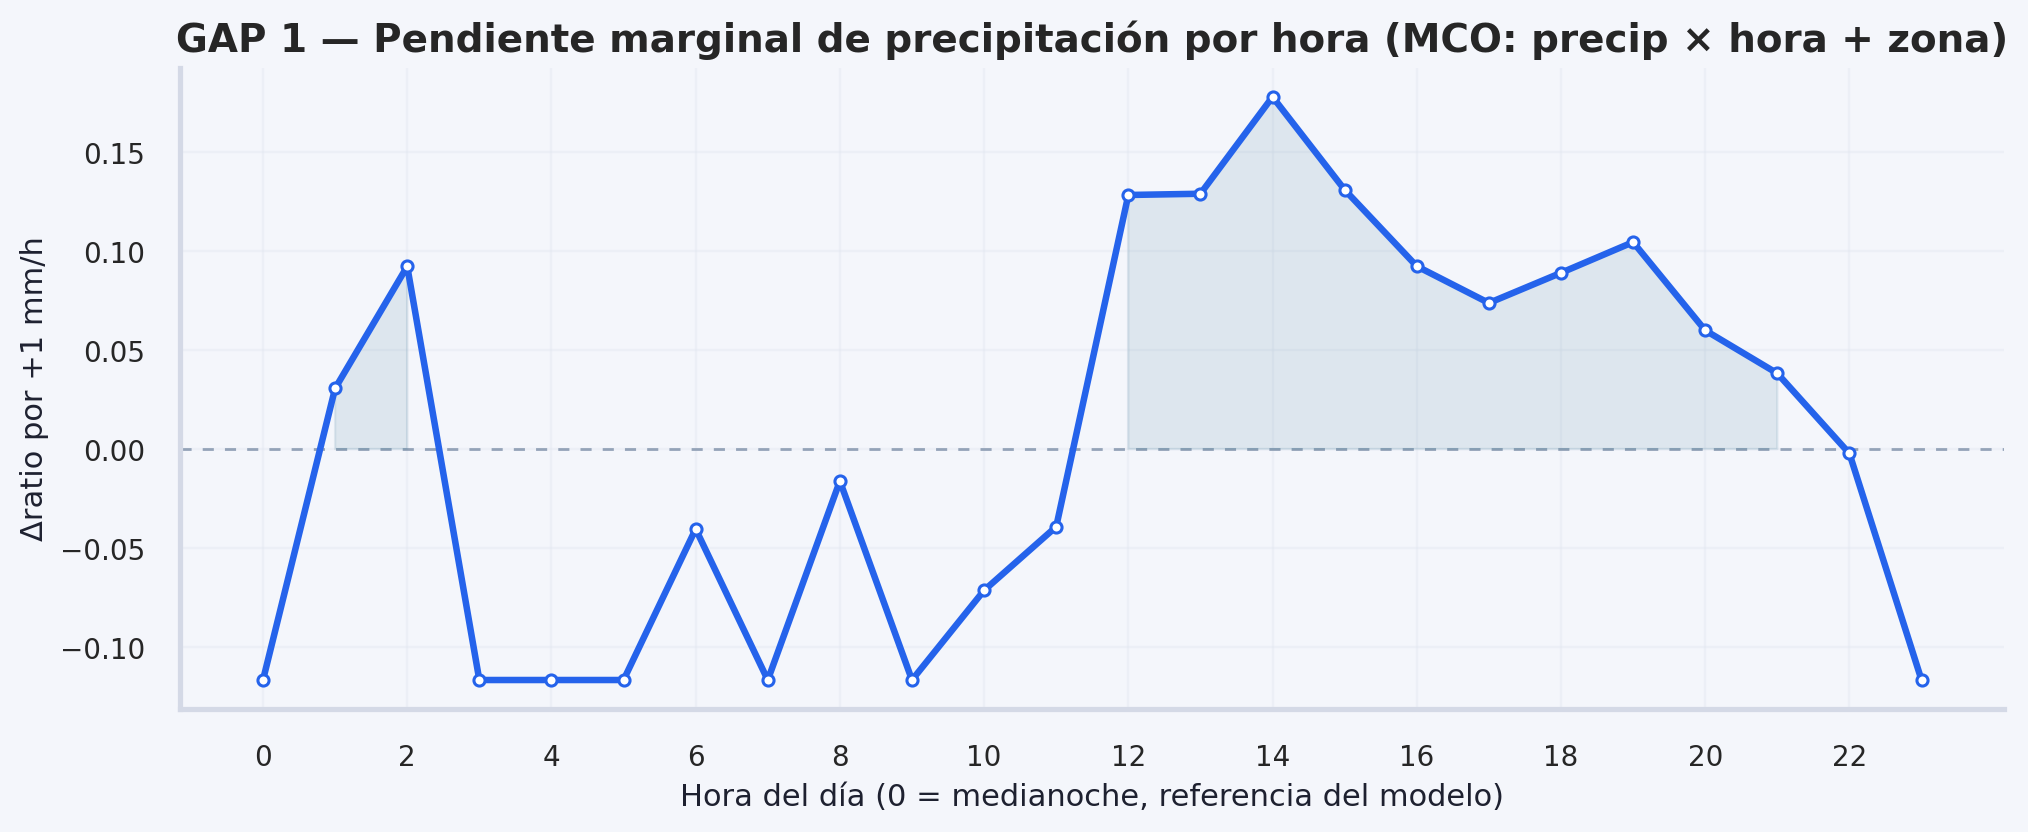
\includegraphics[width=\linewidth,height=0.70\textheight,keepaspectratio]{../modulo1_diagnostico/figures/gap1_precip_marginal_por_hora.png}
  \par
  \endgroup
  \begin{piegrafica}
  Con interacción precipitación$\times$hora, la \textbf{pendiente marginal} de +1~mm/h varía por franja. El gráfico resume $\Delta\text{ratio}$ por hora (referencia \texttt{HOUR}=0).

  Frase tipo negocio (notebook): a las 14:00, +1~mm/h se asocia a $\approx +0{,}178$ en \texttt{ratio} (lectura asociativa).
  \end{piegrafica}
\end{frame}

\begin{frame}[t]{GAP 1 — Tabla: $\Delta$\texttt{ratio} por +1~mm/h (horas 0--11)}
  \begingroup
  \centering
  \small
  \renewcommand{\arraystretch}{1.12}
  \begin{tabular}{@{}lrrrrrr@{}}
    \toprule
    \texttt{HOUR} & 0 & 1 & 2 & 3 & 4 & 5 \\
    \midrule
    $\Delta$\texttt{ratio} & $-0{,}117$ & $+0{,}031$ & $+0{,}092$ & $-0{,}117$ & $-0{,}117$ & $-0{,}117$ \\
    \midrule
    \texttt{HOUR} & 6 & 7 & 8 & 9 & 10 & 11 \\
    \midrule
    $\Delta$\texttt{ratio} & $-0{,}040$ & $-0{,}117$ & $-0{,}016$ & $-0{,}117$ & $-0{,}071$ & $-0{,}039$ \\
    \bottomrule
  \end{tabular}
  \par
  \endgroup
  \begin{piegraficafoot}
  Valores del MCO con interacción precipitación$\times$\texttt{HOUR} (\texttt{HOUR}${}=0$ referencia). Mismos números que imprime el notebook.
  \end{piegraficafoot}
\end{frame}

\begin{frame}[t]{GAP 1 — Tabla: $\Delta$\texttt{ratio} por +1~mm/h (horas 12--23)}
  \begingroup
  \centering
  \small
  \renewcommand{\arraystretch}{1.12}
  \begin{tabular}{@{}lrrrrrr@{}}
    \toprule
    \texttt{HOUR} & 12 & 13 & 14 & 15 & 16 & 17 \\
    \midrule
    $\Delta$\texttt{ratio} & $+0{,}128$ & $+0{,}129$ & $+0{,}178$ & $+0{,}131$ & $+0{,}092$ & $+0{,}074$ \\
    \midrule
    \texttt{HOUR} & 18 & 19 & 20 & 21 & 22 & 23 \\
    \midrule
    $\Delta$\texttt{ratio} & $+0{,}089$ & $+0{,}105$ & $+0{,}060$ & $+0{,}038$ & $-0{,}002$ & $-0{,}117$ \\
    \bottomrule
  \end{tabular}
  \par
  \endgroup
  \begin{piegraficafoot}
  Pico marginal estimado en la hora \textbf{14} del panel; varias horas comparten el coeficiente de referencia ($-0{,}117$) por construcción del modelo.
  \end{piegraficafoot}
\end{frame}

\begin{frame}{P2b — Tabla: saturación y CV(\texttt{ORDERS}) por tramo de \texttt{ratio}}
  \begingroup
  \footnotesize
  \centering
  \renewcommand{\arraystretch}{1.15}
  \begin{tabular}{@{}lrrr@{}}
    \toprule
    \textbf{Tramo} & $n$ & $p_{\text{saturación}}$ & CV(\texttt{ORDERS}) \\
    \midrule
    $<0{,}9$      & 5780 & $0{,}0000$ & $1{,}1828$ \\
    $0{,}9$--$1{,}2$ & 2422 & $0{,}0000$ & $0{,}7761$ \\
    $1{,}2$--$1{,}5$ &  851 & $0{,}0000$ & $0{,}5082$ \\
    $1{,}5$--$1{,}8$ &  514 & $0{,}0000$ & $0{,}3616$ \\
    $>1{,}8$      &  513 & $1{,}0000$ & $0{,}3685$ \\
    \bottomrule
  \end{tabular}
  \par
  \endgroup

  \begin{piegrafica}
  Proxy de ``estrés'' por bandas de \texttt{ratio}. Solo el tramo $>1{,}8$ coincide con saturación operativa del caso. El CV de pedidos sirve como señal de inestabilidad.
  \end{piegrafica}
\end{frame}

\begin{frame}{P2b — Estrés por tramo de \texttt{ratio}}
  \begingroup
  \centering
  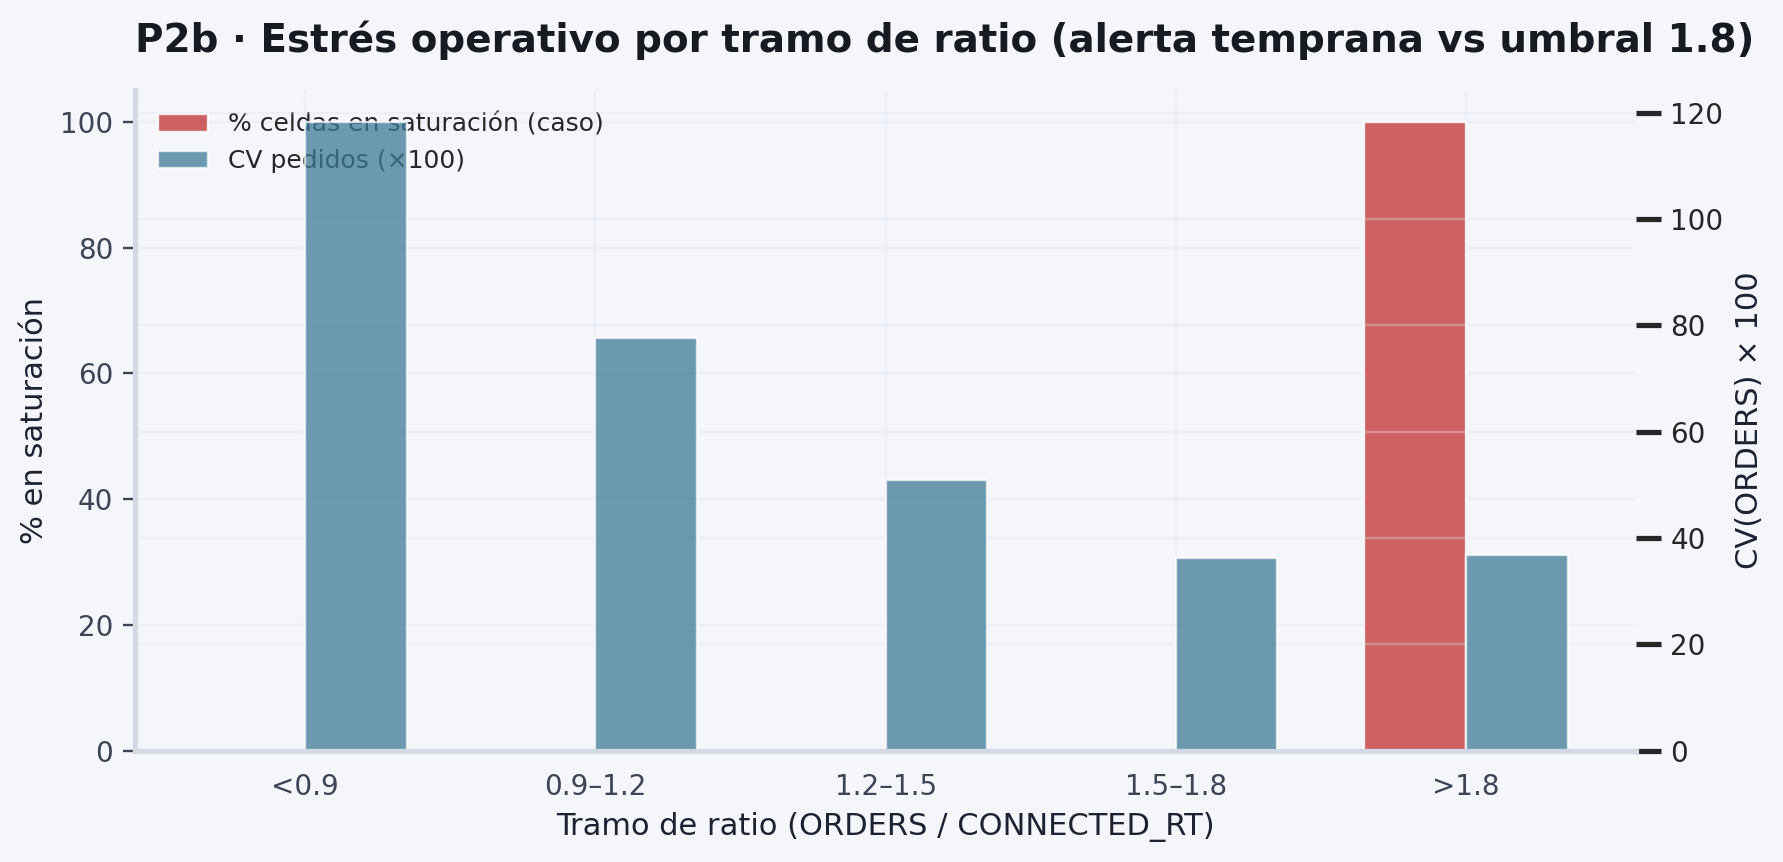
\includegraphics[width=\linewidth,height=0.70\textheight,keepaspectratio]{../modulo1_diagnostico/figures/p2_ratio_tramos_ops.png}
  \par
  \endgroup
  \begin{piegrafica}
  Las barras visualizan la misma lógica que la tabla: cómo cambia la fracción ya en saturación y la variabilidad de \texttt{ORDERS} al moverse el \texttt{ratio} por bandas.
  \end{piegrafica}
\end{frame}

\subsection{Sensibilidad por zona, riesgo y agregados (P3--GAP5)}

\begin{frame}{P3 — Coef.\ precipitación por zona (MCO estratificado, 14 zonas)}
  \begingroup
  \scriptsize
  \centering
  \renewcommand{\arraystretch}{1.08}
  \begin{tabular}{@{}lr@{}}
    \toprule
    \textbf{Zona} & $\beta_{\text{precip}}$ \\
    \midrule
    Santiago            & $0{,}190569$ \\
    Carretera Nacional  & $0{,}131460$ \\
    Santa Catarina      & $0{,}103332$ \\
    MTY Apodaca Huinalá & $0{,}085885$ \\
    Independencia       & $0{,}073652$ \\
    San Pedro           & $0{,}068153$ \\
    Apodaca Centro      & $0{,}065663$ \\
    Escobedo            & $0{,}063273$ \\
    Centro              & $0{,}062092$ \\
    San Nicolás         & $0{,}059934$ \\
    La Fe               & $0{,}059660$ \\
    MTY Guadalupe       & $0{,}058108$ \\
    Cumbres Poniente    & $0{,}052032$ \\
    Mitras Centro       & $0{,}049596$ \\
    \bottomrule
  \end{tabular}
  \par
  \endgroup

  \begin{piegrafica}
  Por zona: \texttt{ratio} $\sim$ precip.\ + \texttt{C(HOUR)} + \texttt{C(dow)}. Orden por magnitud de $\beta$ (mismo criterio que el gráfico P3 del notebook).
  \end{piegrafica}
\end{frame}

\begin{frame}{P3 — Sensibilidad del \texttt{ratio} a la lluvia por zona}
  \begingroup
  \centering
  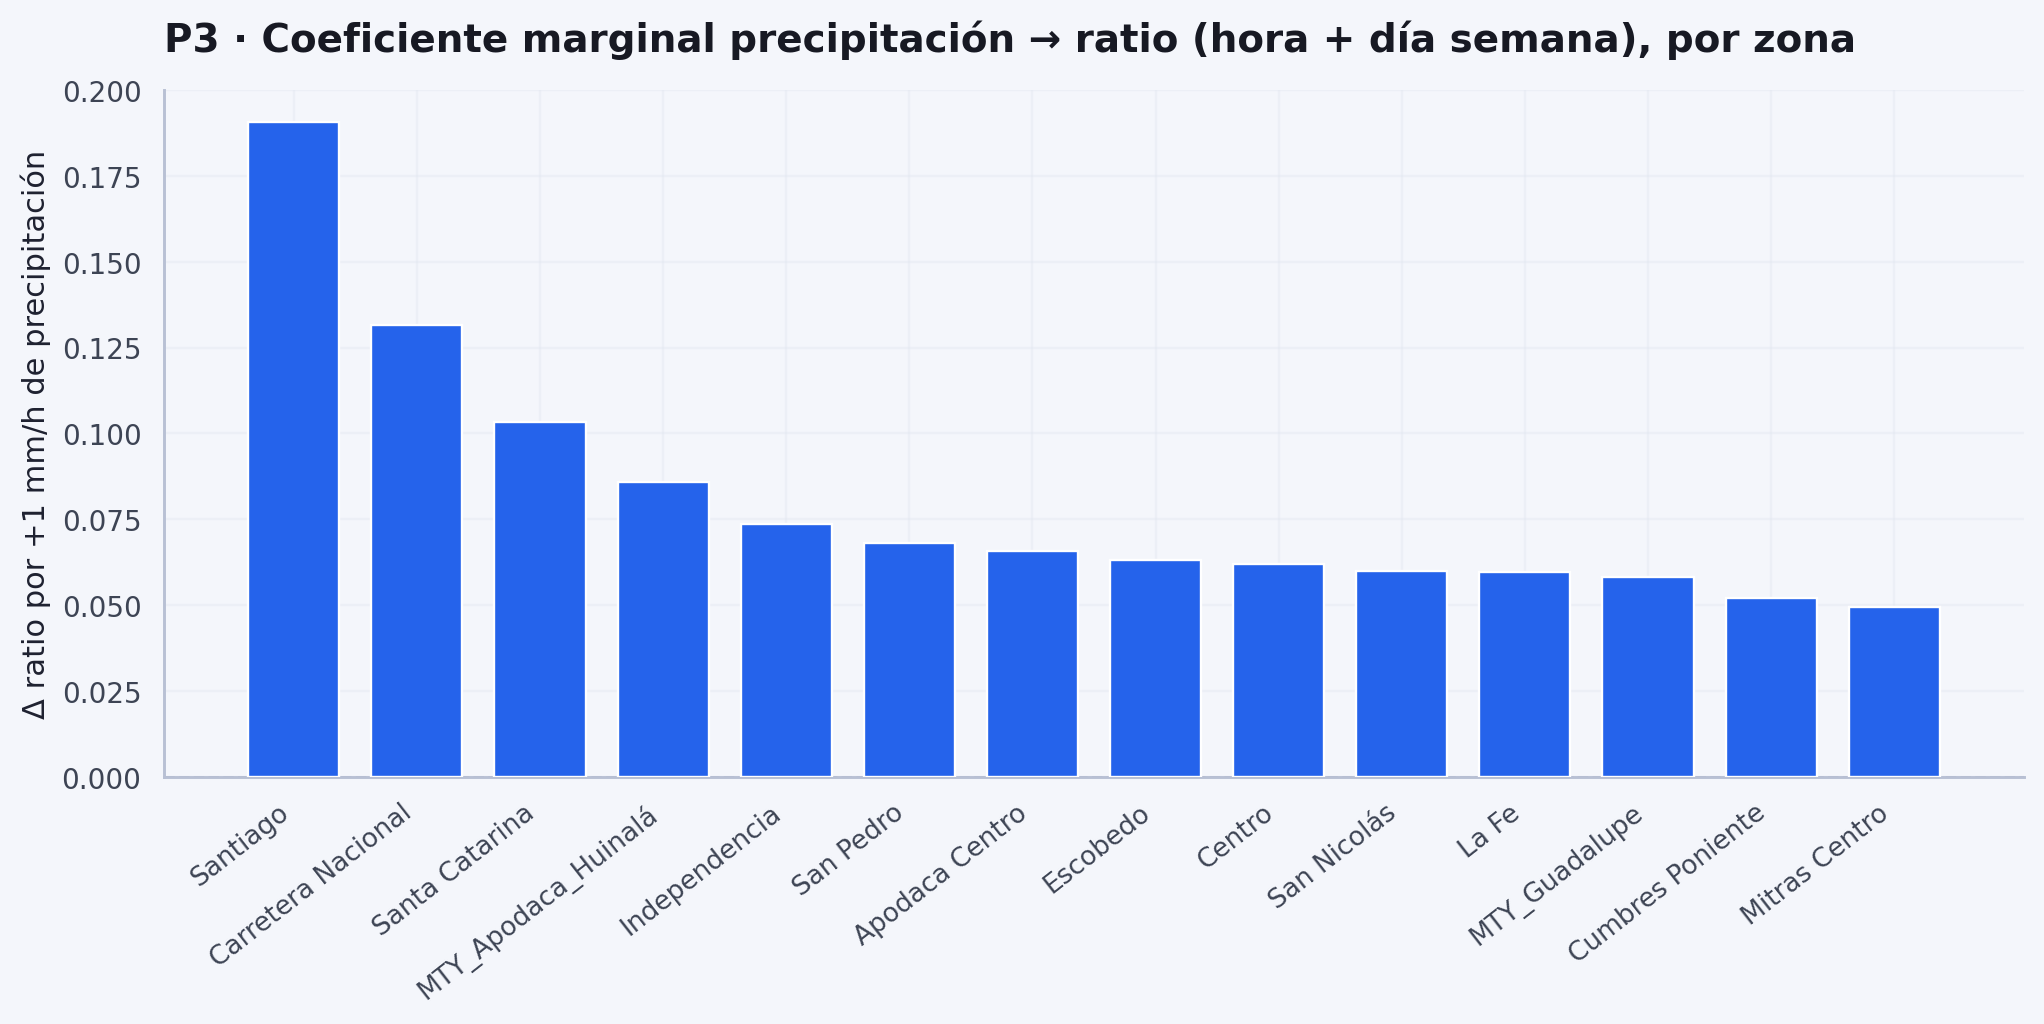
\includegraphics[width=\linewidth,height=0.70\textheight,keepaspectratio]{../modulo1_diagnostico/figures/p3_sensibilidad_zona.png}
  \par
  \endgroup
  \begin{piegrafica}
  El gráfico ordena territorios por magnitud del coeficiente marginal de precipitación (misma especificación dentro de cada \texttt{ZONE}).
  \end{piegrafica}
\end{frame}

\begin{frame}{P4 — Earnings diario vs fracción en saturación}
  \begingroup
  \centering
  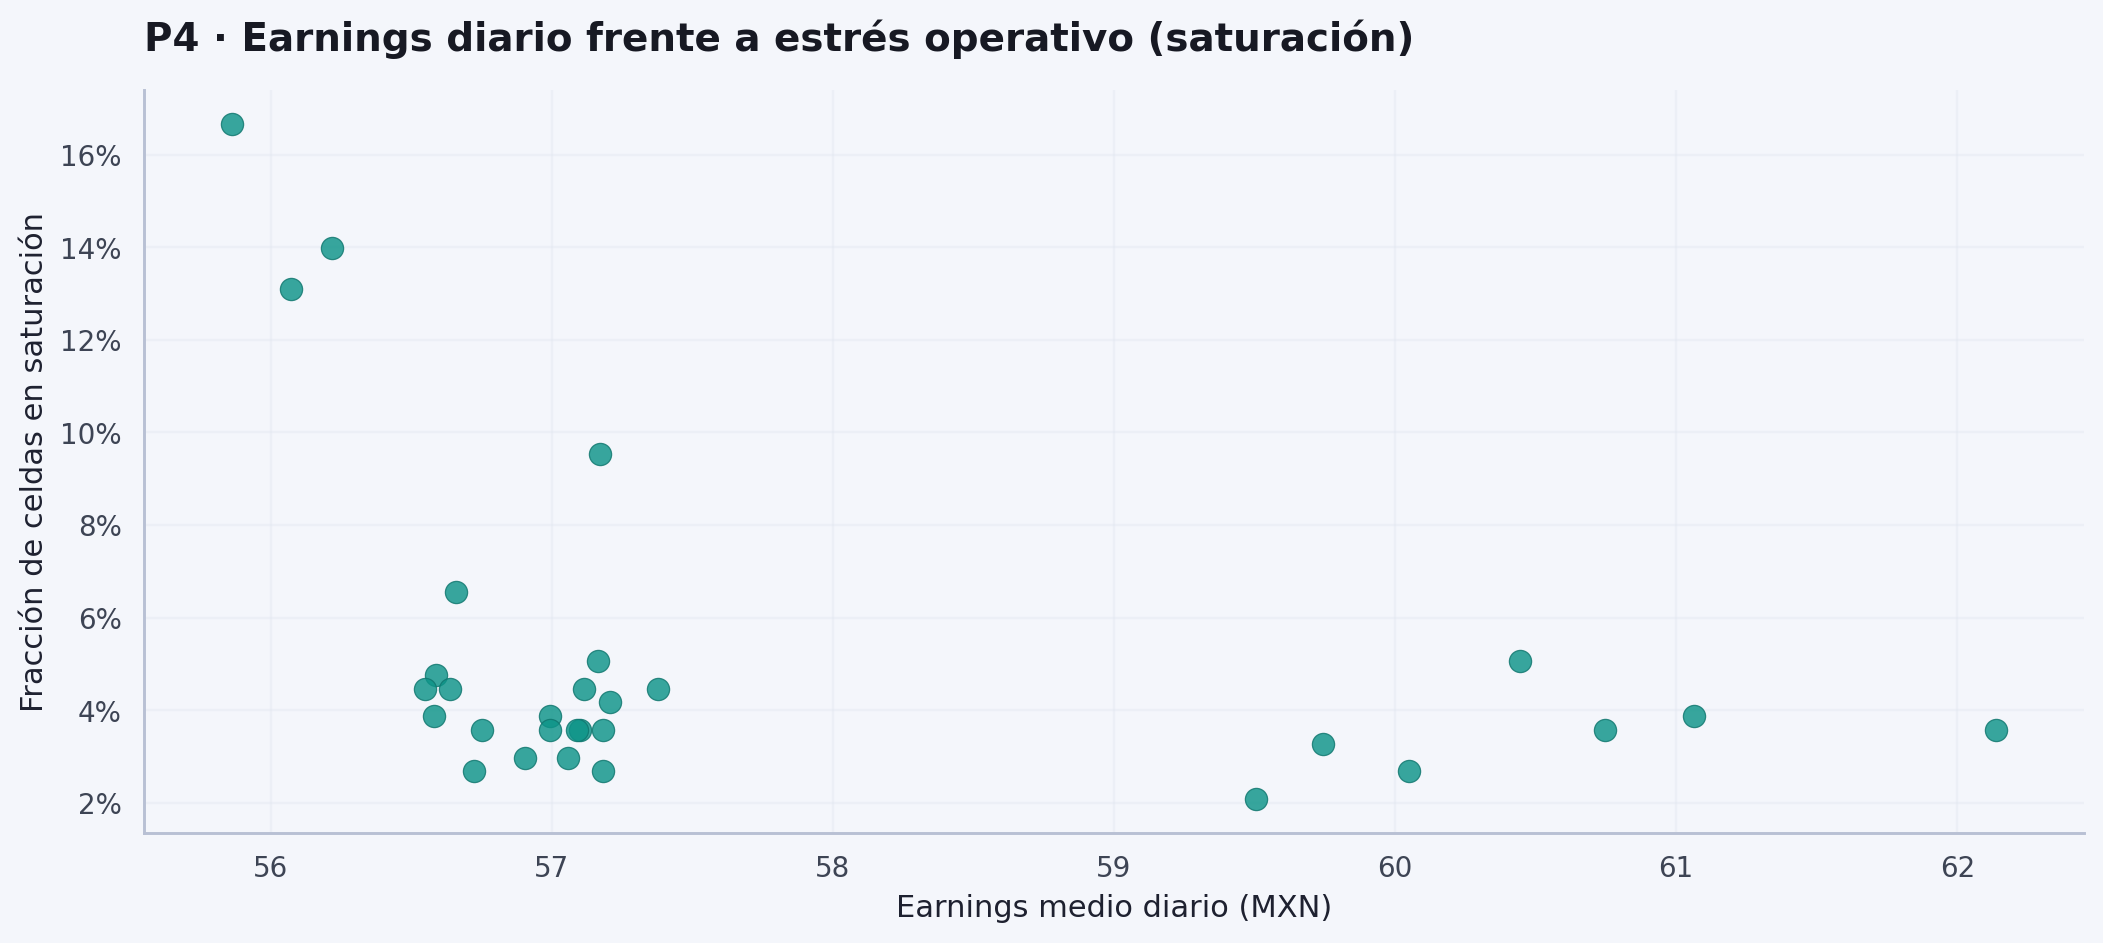
\includegraphics[width=\linewidth,height=0.70\textheight,keepaspectratio]{../modulo1_diagnostico/figures/p4_earnings_vs_estres.png}
  \par
  \endgroup
  \begin{piegrafica}
  Agrega por \textbf{día}: earnings medio frente a fracción de celdas en saturación. Sirve para ver días ``caros'' y estresados.

  Mezclar solo a nivel día puede confundir demanda e incentivos (véase GAP~4).
  \end{piegrafica}
\end{frame}

\begin{frame}{P4 — Top 10 días por fracción en saturación (\texttt{sat\_frac})}
  \begingroup
  \centering
  \scriptsize
  \renewcommand{\arraystretch}{1.05}
  \begin{tabular}{@{}lrrrr@{}}
    \toprule
    \textbf{Fecha} & earn.\ med. & \texttt{sat\_frac} & \texttt{sobre\_frac} & \texttt{ratio} med. \\
    \midrule
    2024-03-28 & $55{,}86$ & $0{,}1667$ & $0{,}1994$ & $1{,}103$ \\
    2024-03-08 & $56{,}22$ & $0{,}1399$ & $0{,}2173$ & $0{,}976$ \\
    2024-03-25 & $56{,}07$ & $0{,}1310$ & $0{,}2143$ & $0{,}896$ \\
    2024-03-05 & $57{,}17$ & $0{,}0952$ & $0{,}2054$ & $0{,}980$ \\
    2024-03-27 & $56{,}66$ & $0{,}0655$ & $0{,}2143$ & $0{,}809$ \\
    2024-03-14 & $60{,}44$ & $0{,}0506$ & $0{,}2798$ & $0{,}746$ \\
    2024-03-16 & $57{,}17$ & $0{,}0506$ & $0{,}2202$ & $0{,}800$ \\
    2024-03-01 & $56{,}59$ & $0{,}0476$ & $0{,}1964$ & $0{,}831$ \\
    2024-03-18 & $56{,}64$ & $0{,}0446$ & $0{,}2024$ & $0{,}814$ \\
    2024-03-26 & $56{,}55$ & $0{,}0446$ & $0{,}2173$ & $0{,}817$ \\
    \bottomrule
  \end{tabular}
  \par
  \endgroup
  \begin{piegraficafoot}
  Agregación diaria del notebook. \textbf{p75 earn + p75 estrés:} solo 2024-03-14. \textbf{p75 earn + p75 sobre-oferta:} 2024-03-03, 07, 14, 22 (detalle en consola del notebook).
  \end{piegraficafoot}
\end{frame}

\begin{frame}{GAP 4 — Horas con mayor $\Delta P(\text{sat})$ (alto $-$ bajo \texttt{EARNINGS}, misma hora)}
  \begingroup
  \footnotesize
  \centering
  \renewcommand{\arraystretch}{1.12}
  \begin{tabular}{@{}crrr@{}}
    \toprule
    \textbf{Hora} & $P_{\text{sat}}(\ge\text{med.})$ & $P_{\text{sat}}(<\text{med.})$ & \textbf{diff} \\
    \midrule
    16 & $0{,}0142$ & $0{,}0000$ & $+0{,}0142$ \\
    15 & $0{,}0095$ & $0{,}0000$ & $+0{,}0095$ \\
    18 & $0{,}0095$ & $0{,}0000$ & $+0{,}0095$ \\
    17 & $0{,}0142$ & $0{,}0048$ & $+0{,}0094$ \\
    \bottomrule
  \end{tabular}
  \par
  \endgroup

  \begin{piegrafica}
  Dentro de cada \texttt{HOUR}, se compara saturación entre filas con \texttt{EARNINGS} alto vs bajo (split por mediana en esa hora). Si diff $\approx 0$, el estrés es similar.

  Si diff $\gg 0$, conviene revisar confusores (zona, lluvia) o la mecánica de incentivos.
  \end{piegrafica}
\end{frame}

\begin{frame}{GAP 4 — Contraste intra-hora (alto vs bajo \texttt{EARNINGS})}
  \begingroup
  \centering
  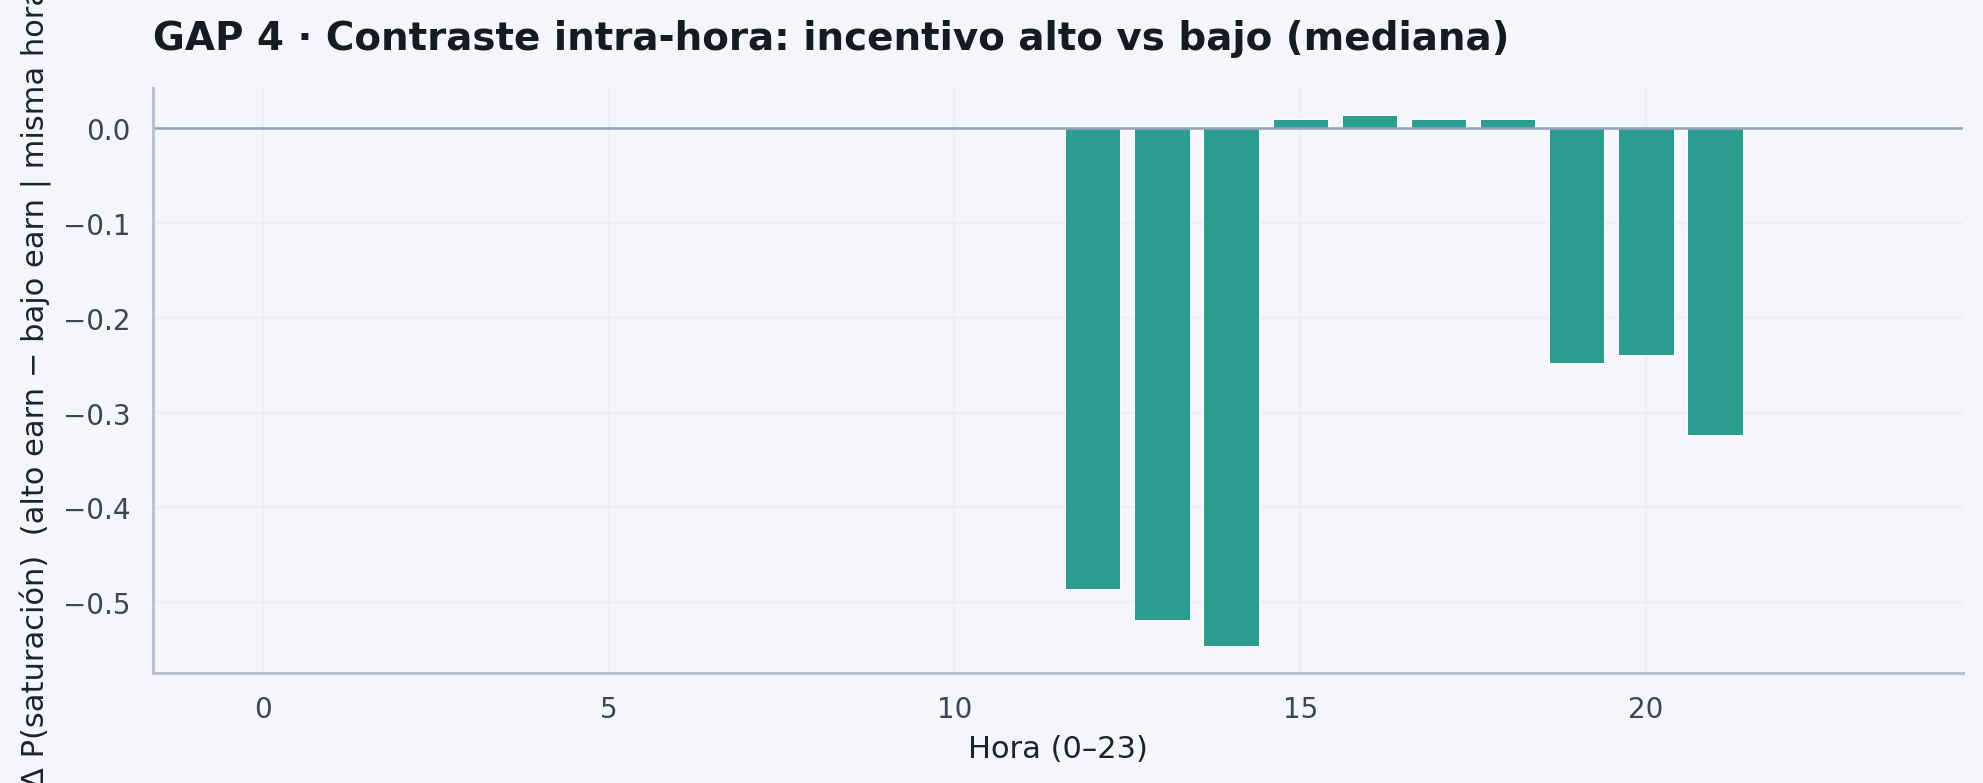
\includegraphics[width=\linewidth,height=0.70\textheight,keepaspectratio]{../modulo1_diagnostico/figures/gap4_p4_counterfactual_misma_hora.png}
  \par
  \endgroup
  \begin{piegrafica}
  La figura resume por hora la diferencia de probabilidad de saturación entre mitades de incentivo. Complementa la tabla de las horas con mayor contraste positivo.
  \end{piegrafica}
\end{frame}

\begin{frame}{GAP 5 — \textit{Risk score} por zona (tabla completa, notebook)}
  \begingroup
  \centering
  \tiny
  \renewcommand{\arraystretch}{1.02}
  \begin{tabular}{@{}lrrrr@{}}
    \toprule
    \textbf{Zona} & \textbf{risk} & $\hat P_{\text{sat}}$ & sens.\ lluvia & demanda \\
    \midrule
    Santa Catarina      & $0{,}0832$ & $0{,}0528$ & $0{,}1033$ & $8{,}50$ \\
    Carretera Nacional  & $0{,}0616$ & $0{,}0597$ & $0{,}1315$ & $5{,}86$ \\
    San Nicolás         & $0{,}0507$ & $0{,}0625$ & $0{,}0599$ & $12{,}53$ \\
    Centro              & $0{,}0420$ & $0{,}0486$ & $0{,}0621$ & $16{,}11$ \\
    Independencia       & $0{,}0404$ & $0{,}0528$ & $0{,}0737$ & $8{,}84$ \\
    MTY Guadalupe       & $0{,}0341$ & $0{,}0611$ & $0{,}0581$ & $11{,}42$ \\
    Apodaca Centro      & $0{,}0292$ & $0{,}0514$ & $0{,}0657$ & $9{,}62$ \\
    San Pedro           & $0{,}0164$ & $0{,}0403$ & $0{,}0682$ & $13{,}67$ \\
    Escobedo            & $0{,}0139$ & $0{,}0500$ & $0{,}0633$ & $7{,}66$ \\
    Cumbres Poniente    & $0{,}0017$ & $0{,}0417$ & $0{,}0520$ & $9{,}96$ \\
    MTY Apodaca Huinalá & $0{,}0000$ & $0{,}0375$ & $0{,}0859$ & $4{,}48$ \\
    La Fe               & $0{,}0000$ & $0{,}0361$ & $0{,}0597$ & $7{,}64$ \\
    Mitras Centro       & $0{,}0000$ & $0{,}0556$ & $0{,}0496$ & $11{,}40$ \\
    Santiago            & $0{,}0000$ & $0{,}0625$ & $0{,}1906$ & $4{,}48$ \\
    \bottomrule
  \end{tabular}
  \par
  \endgroup

  \begin{piegrafica}
  $\text{risk} = \hat P(\text{sat}) \times \text{sensibilidad\_lluvia} \times \text{demanda}$ con factores min--max por columna en el panel (impreso en consola del notebook). Top~3: Santa Catarina, Carretera Nacional, San Nicolás.
  \end{piegrafica}
\end{frame}

\begin{frame}{GAP 5 — \textit{Risk score} por zona}
  \begingroup
  \centering
  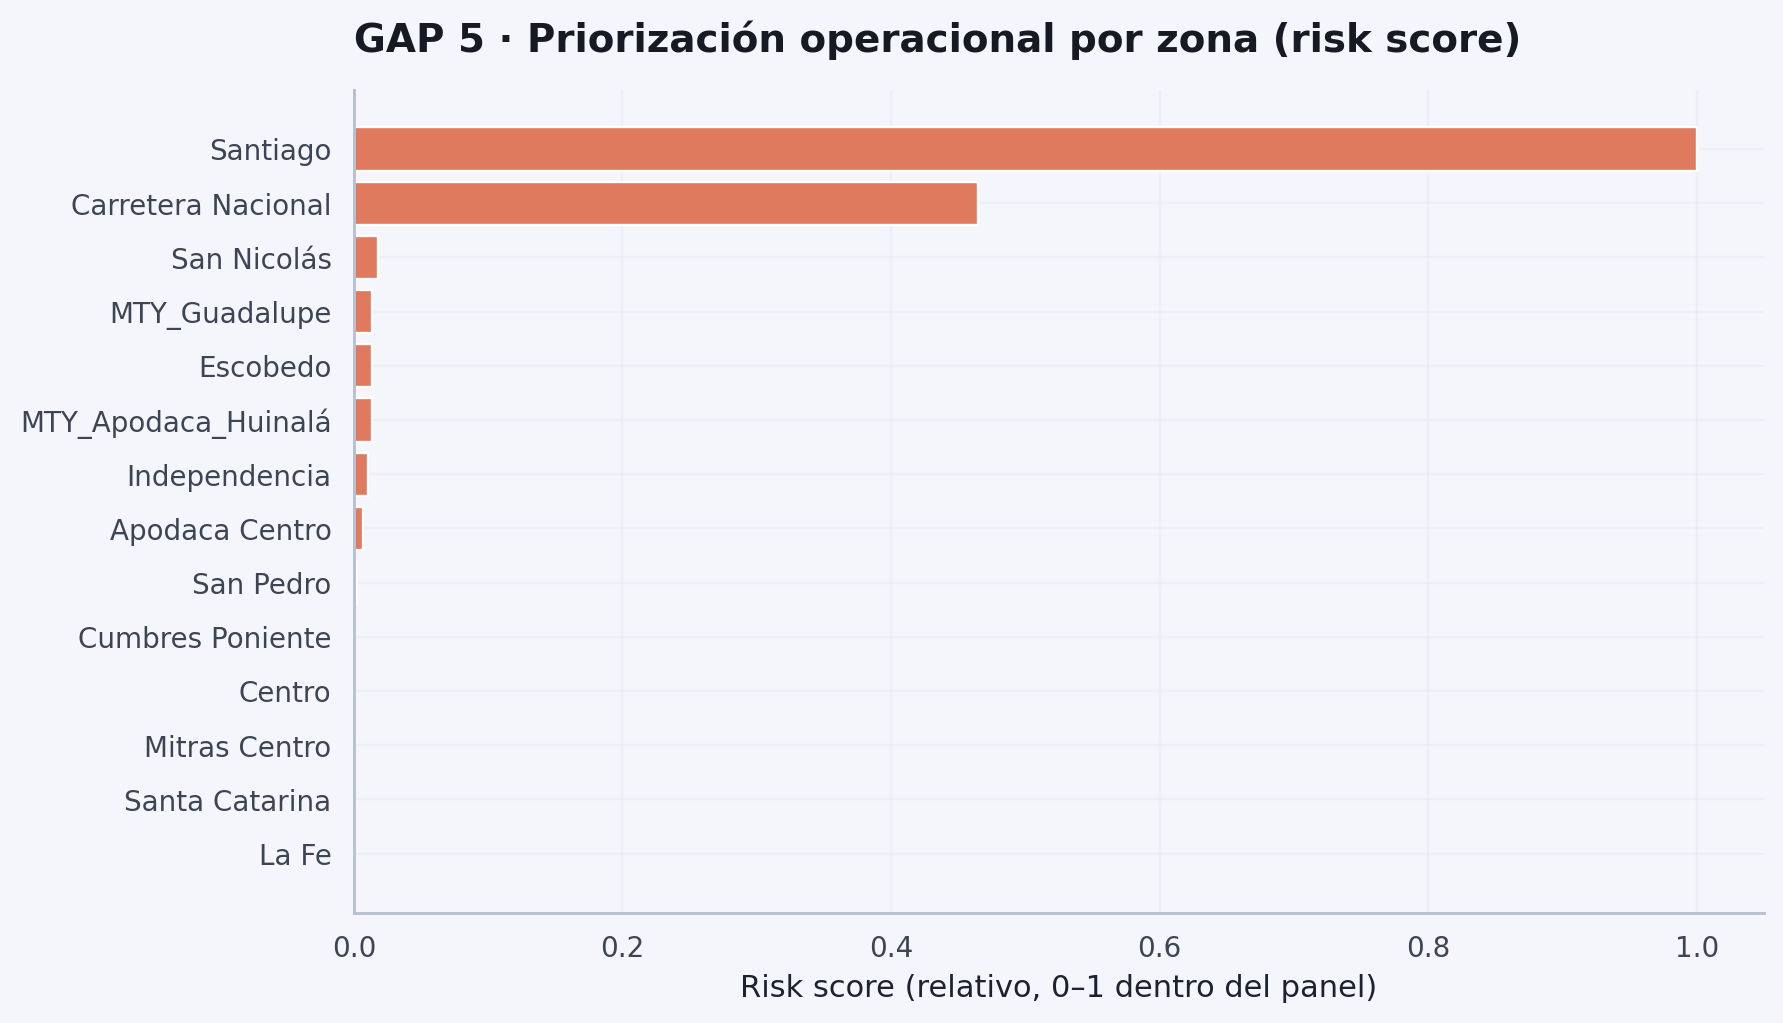
\includegraphics[width=\linewidth,height=0.70\textheight,keepaspectratio]{../modulo1_diagnostico/figures/gap5_risk_score_zonas.png}
  \par
  \endgroup
  \begin{piegrafica}
  Ranking visual coherente con la tabla; escala normalizada para comparar zonas en un solo gráfico.
  \end{piegrafica}
\end{frame}

\begin{frame}{Sensibilidad — mm/h para $\Delta\text{ratio}\approx 0{,}6$ (tabla)}
  \begingroup
  \centering
  \scriptsize
  \renewcommand{\arraystretch}{1.05}
  \begin{tabular}{@{}lrr@{}}
    \toprule
    \textbf{Zona} & $\beta_{\text{precip}}$ & mm/h ($\approx 0{,}6/\beta$) \\
    \midrule
    Santiago            & $0{,}1906$ & $3{,}15$ \\
    Carretera Nacional  & $0{,}1315$ & $4{,}56$ \\
    Santa Catarina      & $0{,}1033$ & $5{,}81$ \\
    MTY Apodaca Huinalá & $0{,}0859$ & $6{,}99$ \\
    Independencia       & $0{,}0737$ & $8{,}15$ \\
    San Pedro           & $0{,}0682$ & $8{,}80$ \\
    Apodaca Centro      & $0{,}0657$ & $9{,}14$ \\
    Escobedo            & $0{,}0633$ & $9{,}48$ \\
    Centro              & $0{,}0621$ & $9{,}66$ \\
    San Nicolás         & $0{,}0599$ & $10{,}01$ \\
    La Fe               & $0{,}0597$ & $10{,}06$ \\
    MTY Guadalupe       & $0{,}0581$ & $10{,}33$ \\
    Cumbres Poniente    & $0{,}0520$ & $11{,}53$ \\
    Mitras Centro       & $0{,}0496$ & $12{,}10$ \\
    \bottomrule
  \end{tabular}
  \par
  \endgroup
  \begin{piegraficafoot}
  Heurística del notebook: $\Delta\text{precip} \approx 0{,}6/\beta$ si $\beta>0$ (banda de \texttt{ratio} $1{,}2\to 1{,}8$). Lectura de orden de magnitud bajo linealidad local.
  \end{piegraficafoot}
\end{frame}

\begin{frame}{Sensibilidad — mm/h (gráfico)}
  \begingroup
  \centering
  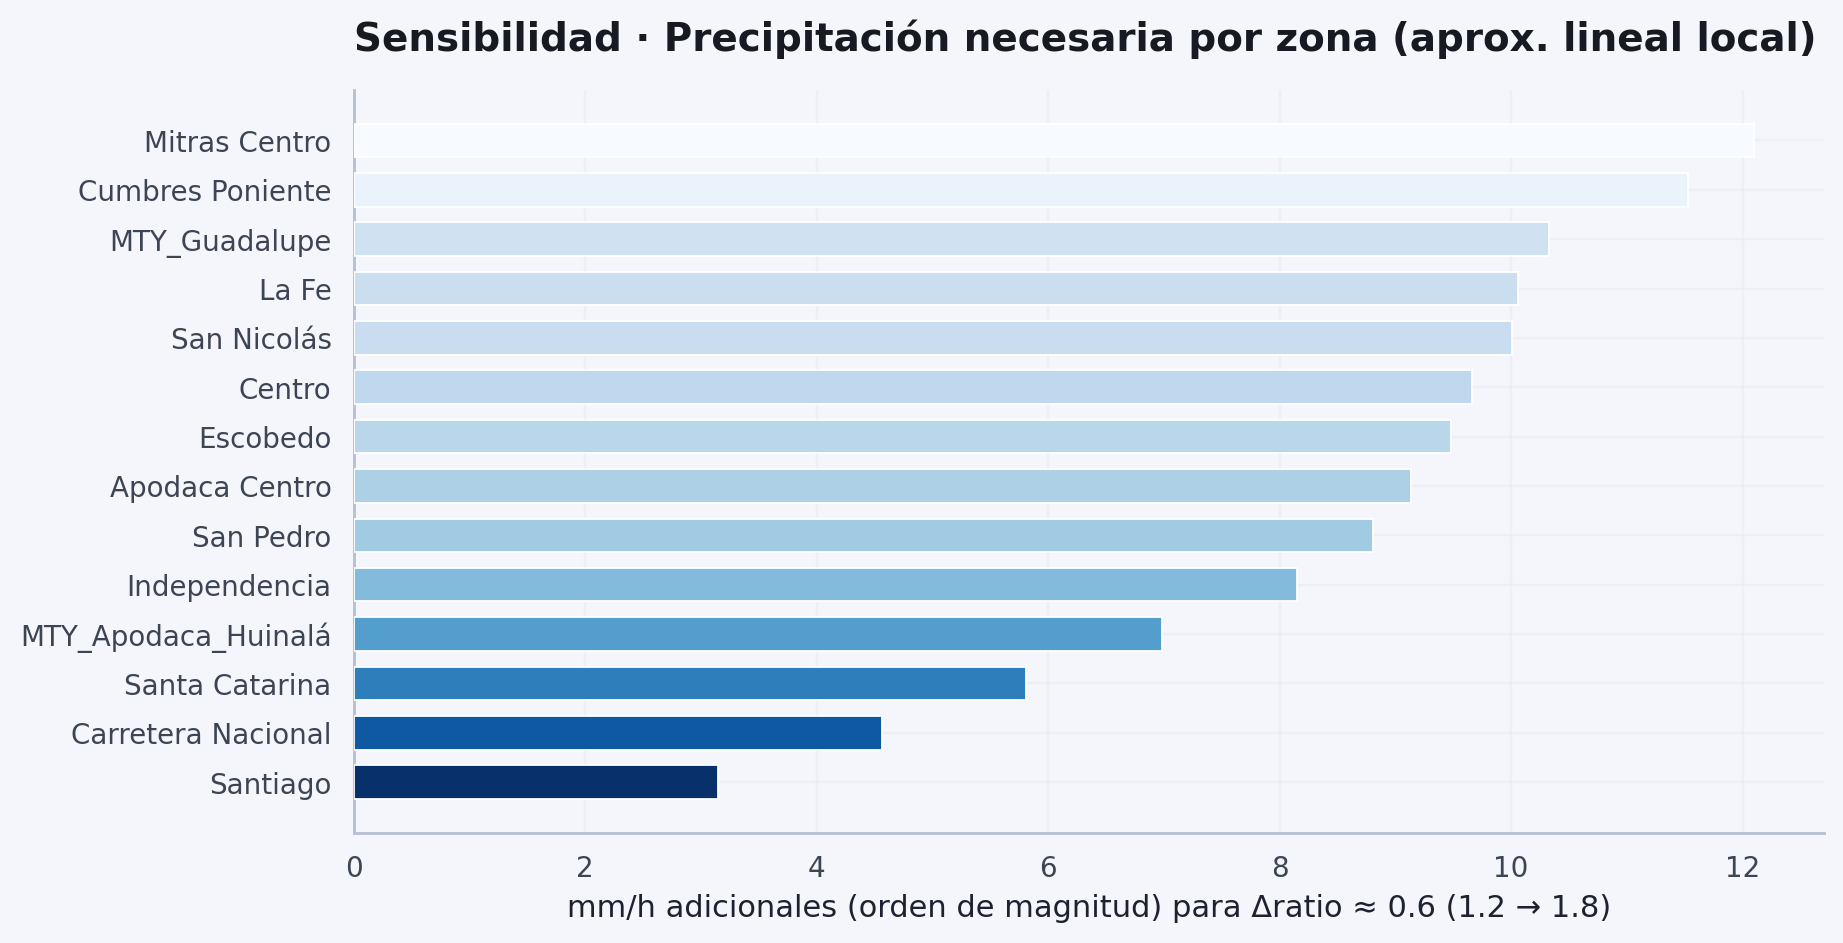
\includegraphics[width=\linewidth,height=0.70\textheight,keepaspectratio]{../modulo1_diagnostico/figures/p_sensitivity_mm_12_to_18.png}
  \par
  \endgroup
  \begin{piegrafica}
  Misma información que la tabla anterior en formato barras horizontales.
  \end{piegrafica}
\end{frame}

\begin{frame}{P6 — Reparto de incentivos (pico por zona)}
  \begingroup
  \centering
  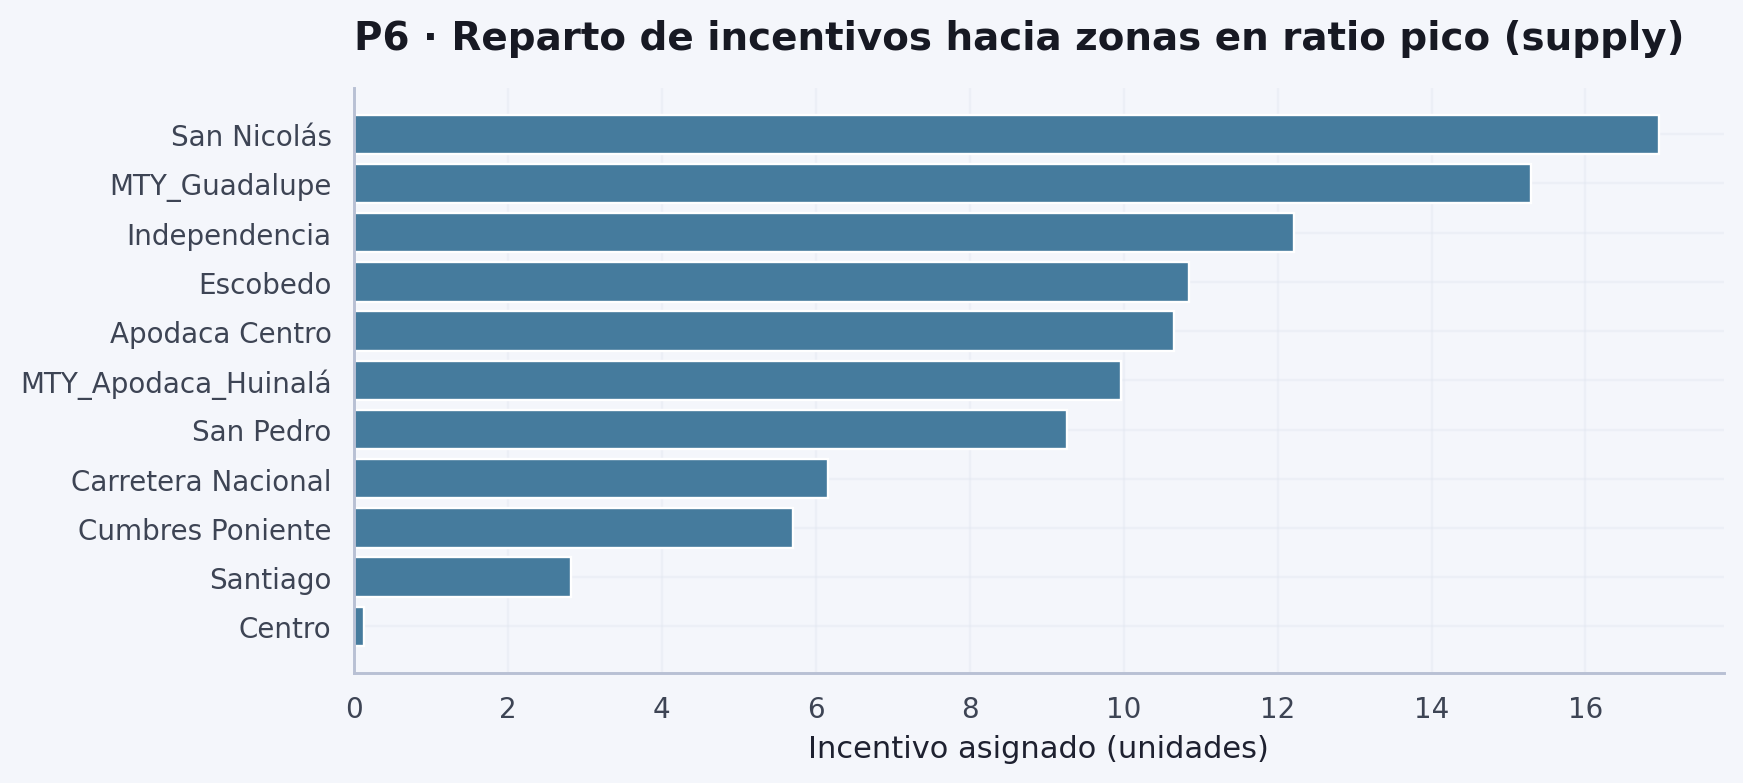
\includegraphics[width=\linewidth,height=0.70\textheight,keepaspectratio]{../modulo1_diagnostico/figures/p6_reparto_incentivos_zonas.png}
  \par
  \endgroup
  \begin{piegrafica}
  Solución de optimización que prioriza atraer oferta hacia zonas más tensionadas en el instante pico, con pesos de riesgo y probabilidad de saturación.

  No sustituye al motor M2 ni a políticas reales de incentivos.
  \end{piegrafica}
\end{frame}

\subsection{Calendario, dispersión exógena y tablas GAP2/3/P5}

\begin{frame}{Calendario — Tests (\texttt{ratio} vs día y festivos MX)}
  \begingroup
  \footnotesize
  \centering
  \renewcommand{\arraystretch}{1.15}
  \begin{tabular}{@{}p{0.30\textwidth}p{0.64\textwidth}@{}}
    \toprule
    \textbf{Test} & \textbf{Resultado (panel)} \\
    \midrule
    Kruskal--Wallis & \texttt{ratio} vs día semana: estad.\ $\approx 6{,}26$, $p \approx 0{,}395$ \\
    Mann--Whitney   & Festivo vs no festivo: $p \approx 0{,}00185$. \newline $n_{\text{fest}}=1008$, $n_{\text{no}}=9072$ \\
    Spearman        & \texttt{ratio} vs índice Lun--Dom: $\rho \approx -0{,}0213$, $p \approx 0{,}032$ \\
    \bottomrule
  \end{tabular}
  \par
  \endgroup

  \begin{piegrafica}
  El día de la semana no muestra diferencias fuertes en el test global. Los festivos sí se asocian a diferencias de \texttt{ratio} (asociativo).

  El Spearman con índice de día es solo exploratorio.
  \end{piegrafica}
\end{frame}

\begin{frame}{Calendario — \texttt{ratio} por día y festivo vs no festivo}
  \begingroup
  \centering
  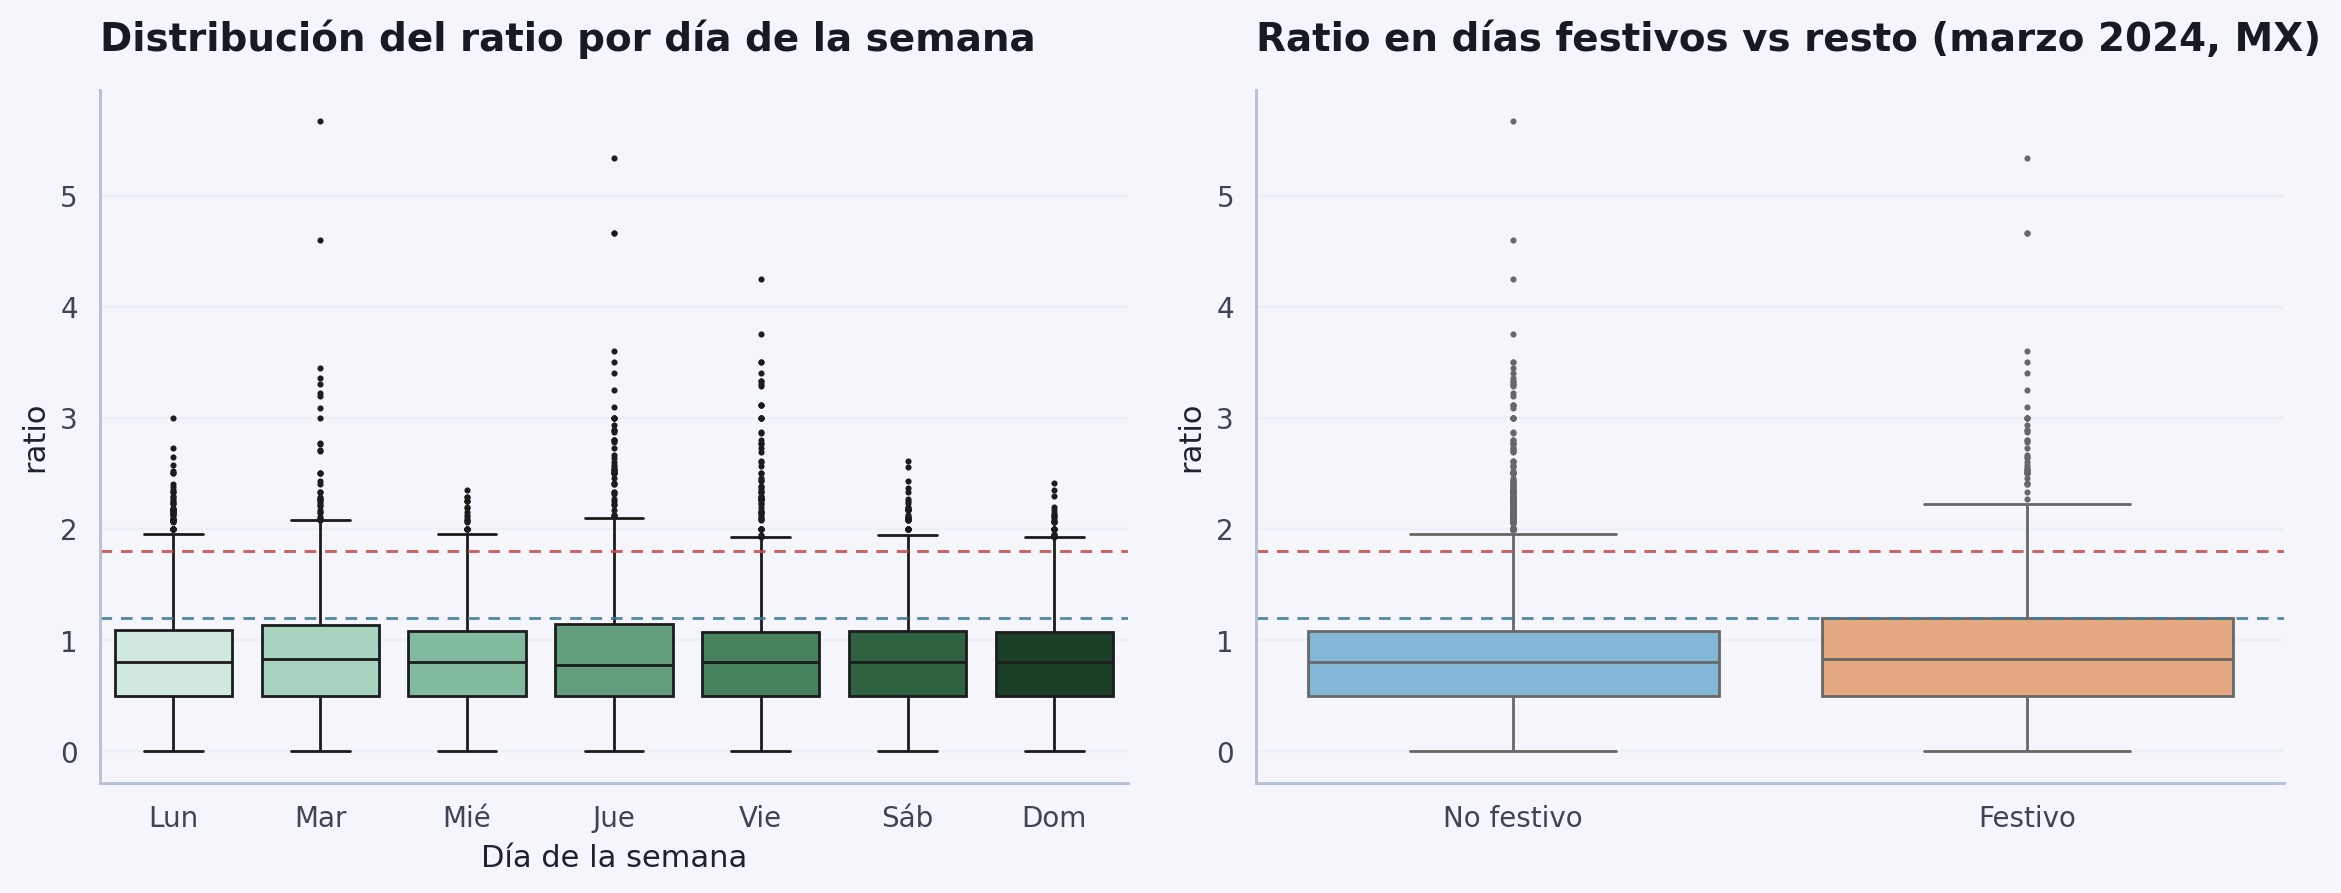
\includegraphics[width=\linewidth,height=0.70\textheight,keepaspectratio]{../modulo1_diagnostico/figures/calendario_ratio_dow_festivos.png}
  \par
  \endgroup
  \begin{piegrafica}
  Boxplots de \texttt{ratio} por día de la semana y comparación festivo / no festivo, coherentes con los contrastes no paramétricos de la lámina anterior.
  \end{piegrafica}
\end{frame}

\begin{frame}{Factores exógenos — precipitación del caso vs \texttt{ratio}}
  \begingroup
  \centering
  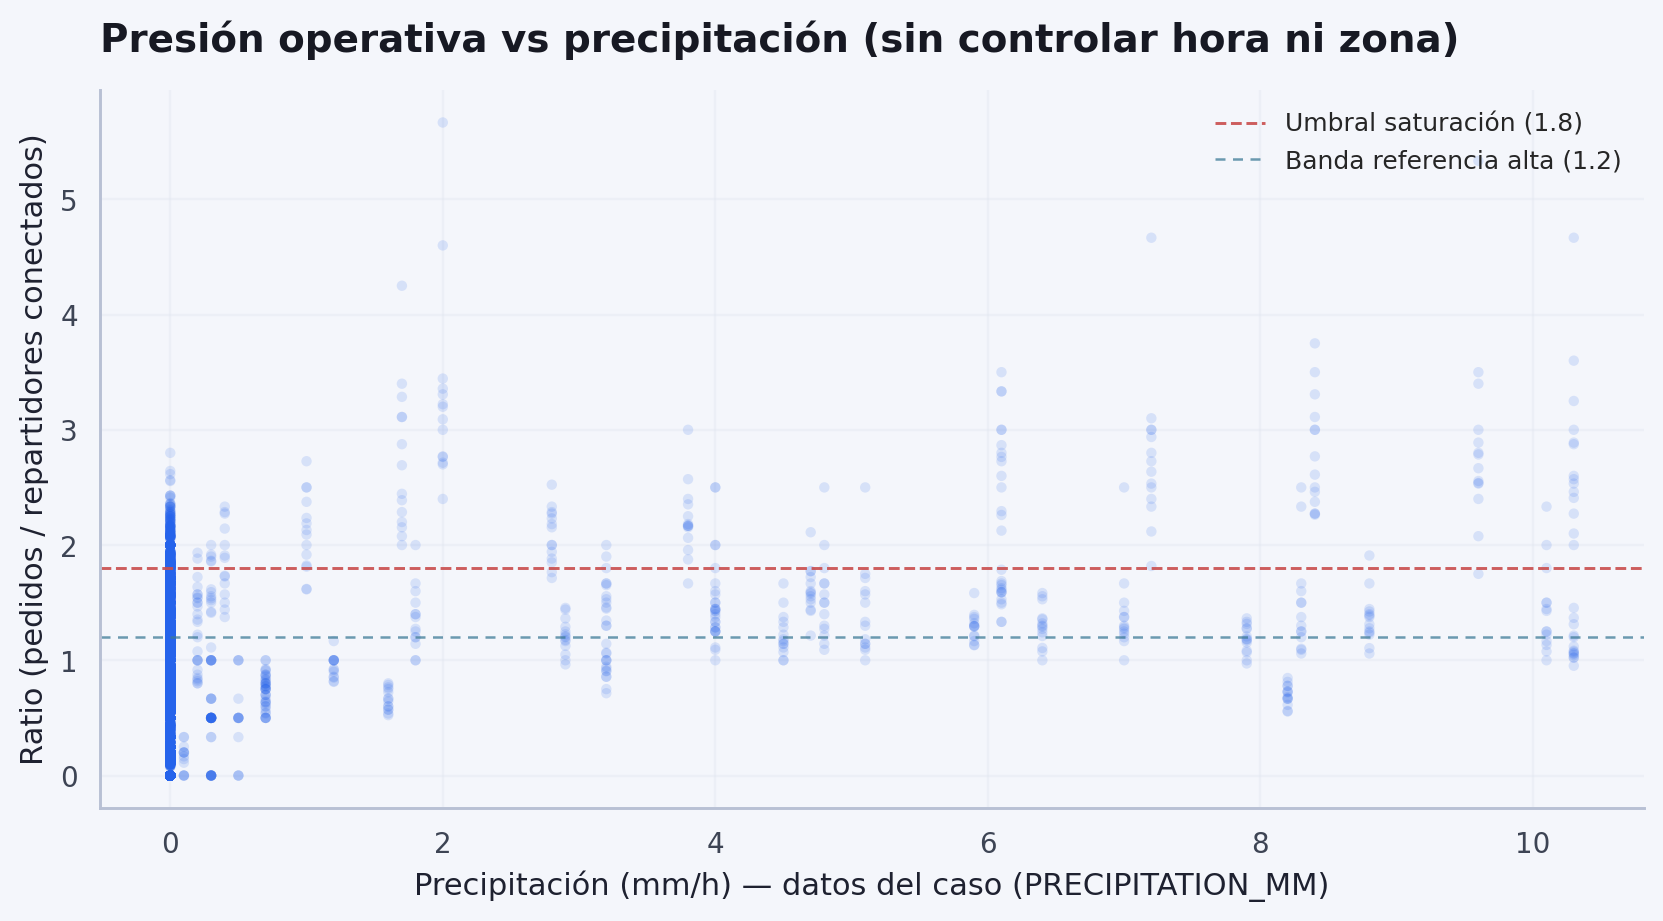
\includegraphics[width=\linewidth,height=0.70\textheight,keepaspectratio]{../modulo1_diagnostico/figures/m1_ratio_vs_precipitation_exog_section.png}
  \par
  \endgroup
  \begin{piegrafica}
  Dispersión \texttt{ratio} vs precipitación del panel; complementa el MCO y extensiones con variables exógenas (temperatura/humedad) cuando existen.

  Spearman precipitación--\texttt{ratio} en panel: $\rho \approx 0{,}2307$.
  \end{piegrafica}
\end{frame}

\begin{frame}{P5 — Spearman \texttt{EARNINGS} vs \texttt{ratio} (panel completo)}
  \begingroup
  \footnotesize
  \centering
  \renewcommand{\arraystretch}{1.2}
  \begin{tabular}{@{}lr@{}}
    \toprule
    \textbf{Contraste} & \textbf{Valor (notebook)} \\
    \midrule
    Spearman global ($n=10\,080$) & $\rho \approx 0{,}0761$ \\
    $p$-valor (dos colas) & $\approx 1{,}95\times 10^{-14}$ \\
    \bottomrule
  \end{tabular}
  \par
  \endgroup

  \begin{piegrafica}
  Correlación de \emph{rangos} (monótona, no lineal) entre tarifa y carga. Complementa Pearson y el MCO con interacción lluvia$\times$\texttt{EARNINGS} en la lámina siguiente.
  \end{piegrafica}
\end{frame}

\begin{frame}{Tablas — oferta, saturación y P5 (mismos datos que el notebook)}
  \begingroup
  \footnotesize
  \centering
  \renewcommand{\arraystretch}{1.22}
  \begin{tabular}{@{}p{0.52\textwidth}r@{}}
    \toprule
    \textbf{Resultado (panel 10\,080 celdas)} & \textbf{Valor} \\
    \midrule
    \multicolumn{2}{@{}l}{\textit{GAP 2 — Oferta} \quad \texttt{CONNECTED\_RT} $\sim$ \texttt{EARNINGS} + precip.\ + \texttt{C(HOUR)} + \texttt{C(ZONE)}} \\
    Coef.\ \texttt{EARNINGS} ($+1$ MXN $\to$ $\Delta$ RT, ceteris paribus) & $+0{,}3401$ \\
    \midrule
    \multicolumn{2}{@{}l}{\textit{GAP 3 — Logit} \quad $P(\texttt{ratio}>1{,}8)$ $\sim$ precip.\ + \texttt{EARNINGS} + \texttt{C(HOUR)} + \texttt{C(ZONE)}} \\
    Pseudo $R^2$ (McFadden) & $0{,}700$ \\
    \midrule
    \multicolumn{2}{@{}l}{\textit{P5 — Interacción} \quad \texttt{ratio} $\sim$ \texttt{EARNINGS}$\times$\texttt{PRECIPITATION\_MM} + \texttt{C(HOUR)} + \texttt{C(ZONE)}} \\
    Coef.\ \texttt{EARNINGS:PRECIPITATION\_MM} & $-0{,}001895$ \\
    $p$-valor (aprox.) & $< 10^{-50}$ \\
    \bottomrule
  \end{tabular}
  \par
  \endgroup

  \begin{piegrafica}
  La oferta (\texttt{CONNECTED\_RT}) responde a incentivos y controles. El logit resume probabilidad de saturación con muchos predictores.

  La interacción P5 indica que la pendiente de \texttt{EARNINGS} sobre el \texttt{ratio} \emph{cambia} con la lluvia (asociativo). Números alineados con el Excel y el notebook \texttt{01\_diagnostico\_operacional.ipynb}.
  \end{piegrafica}
\end{frame}

\subsection{P1 — Frecuencia por hora (una lámina por zona)}

\begin{frame}{P1 · Apodaca Centro}
  \begingroup
  \centering
  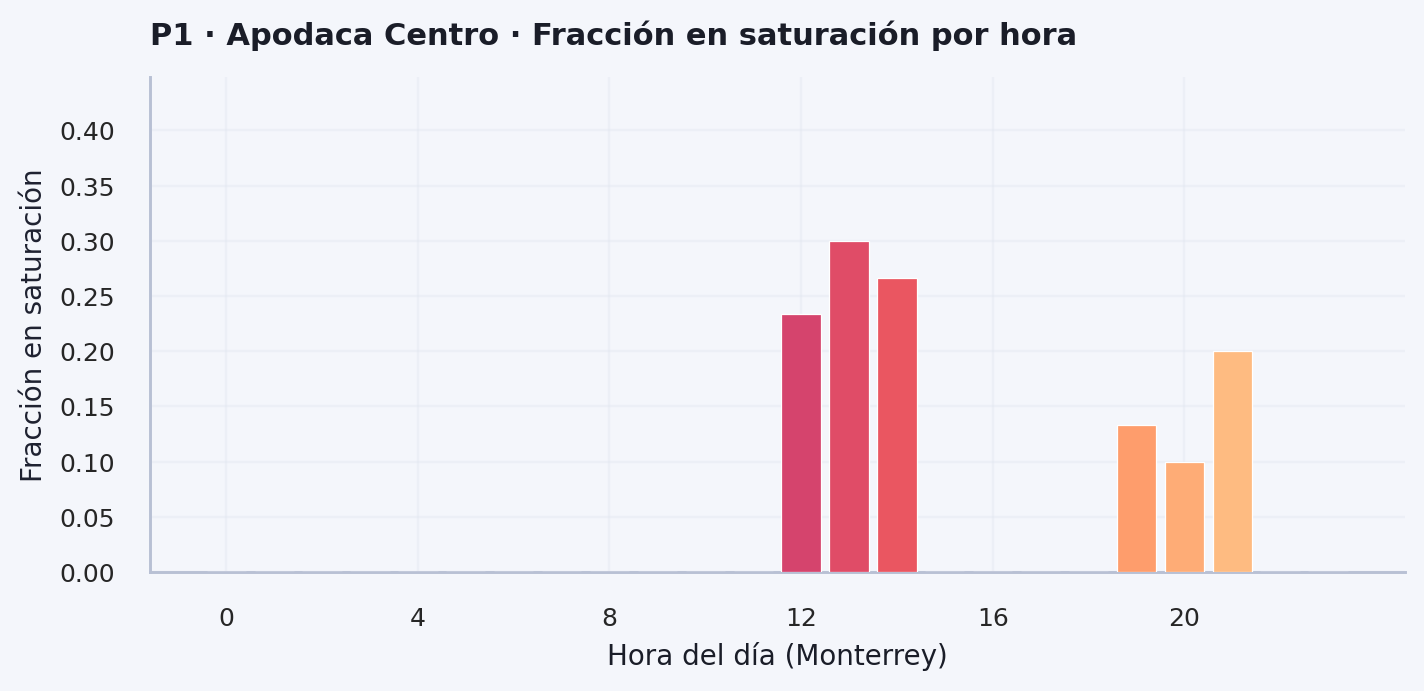
\includegraphics[width=\linewidth,height=0.68\textheight,keepaspectratio]{../modulo1_diagnostico/figures/p1_frecuencia_por_zona/p1_frecuencia_hora__Apodaca_Centro.png}
  \par
  \endgroup
  \pizoneread
\end{frame}

\begin{frame}{P1 · Carretera Nacional}
  \begingroup
  \centering
  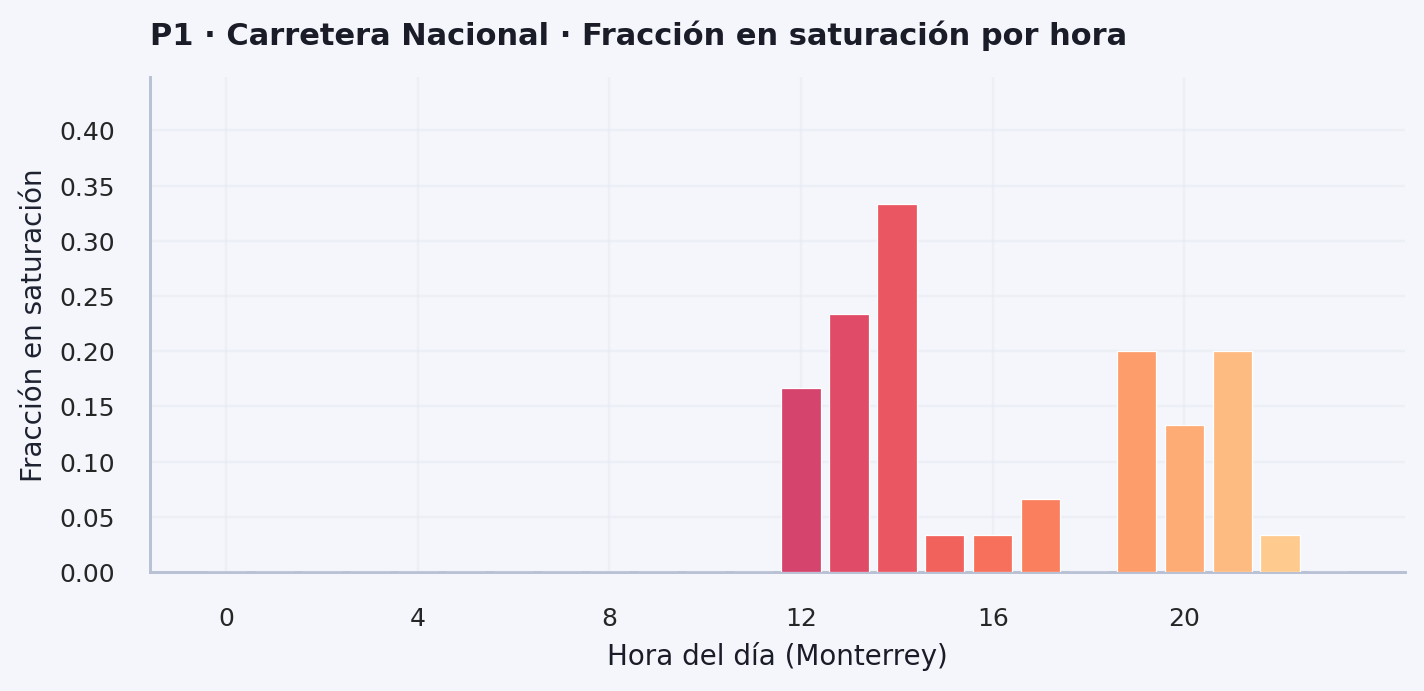
\includegraphics[width=\linewidth,height=0.68\textheight,keepaspectratio]{../modulo1_diagnostico/figures/p1_frecuencia_por_zona/p1_frecuencia_hora__Carretera_Nacional.png}
  \par
  \endgroup
  \pizoneread
\end{frame}

\begin{frame}{P1 · Centro}
  \begingroup
  \centering
  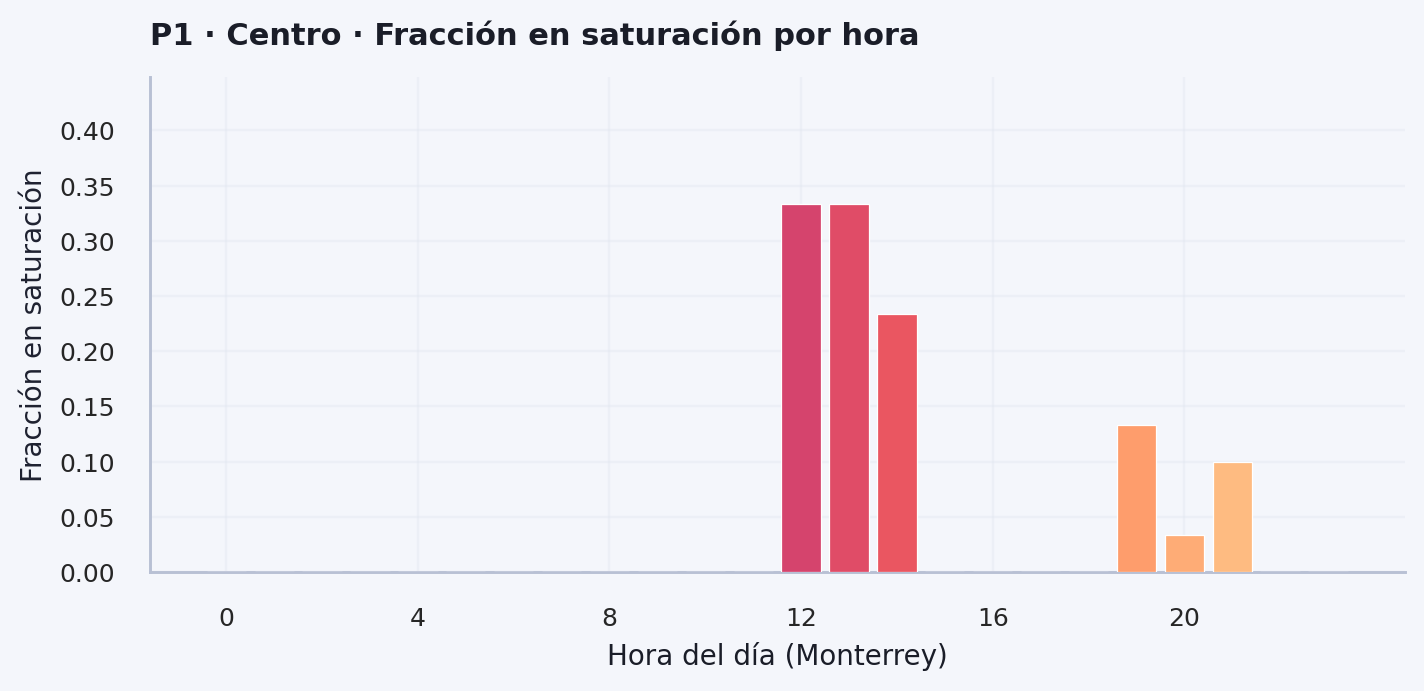
\includegraphics[width=\linewidth,height=0.68\textheight,keepaspectratio]{../modulo1_diagnostico/figures/p1_frecuencia_por_zona/p1_frecuencia_hora__Centro.png}
  \par
  \endgroup
  \pizoneread
\end{frame}

\begin{frame}{P1 · Cumbres Poniente}
  \begingroup
  \centering
  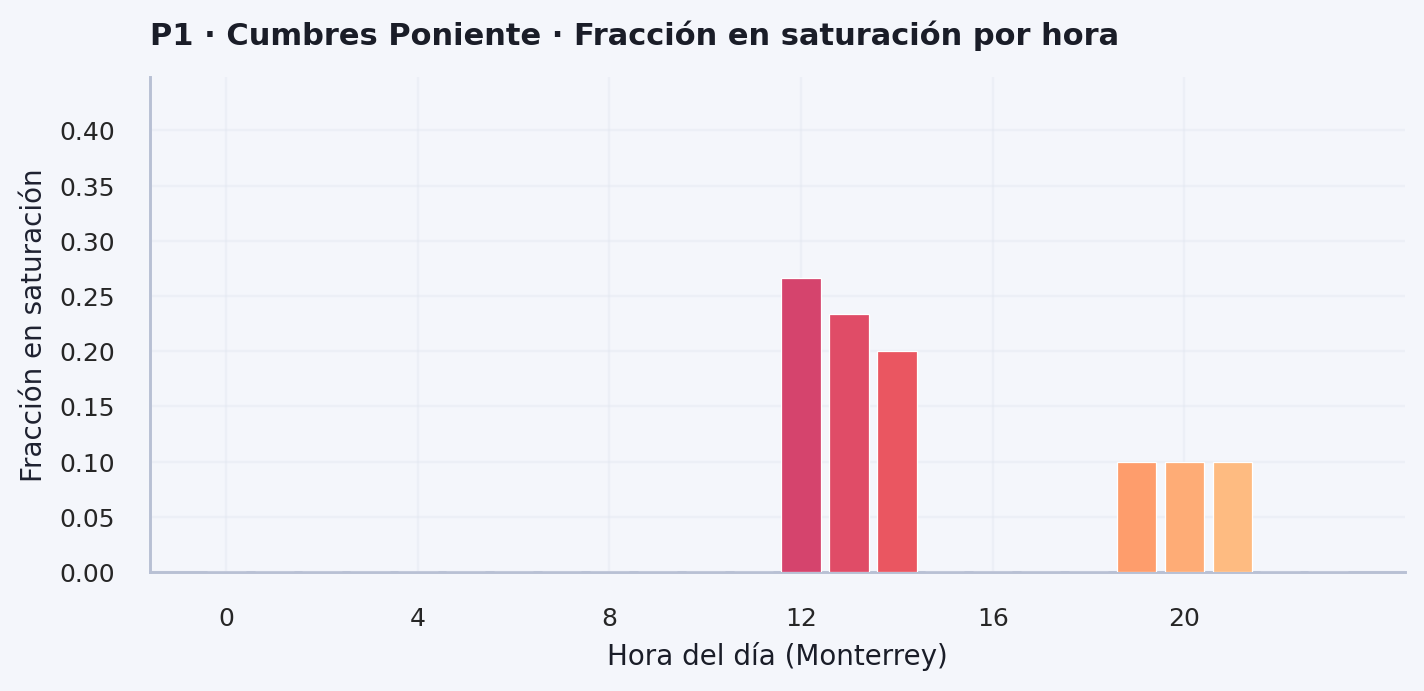
\includegraphics[width=\linewidth,height=0.68\textheight,keepaspectratio]{../modulo1_diagnostico/figures/p1_frecuencia_por_zona/p1_frecuencia_hora__Cumbres_Poniente.png}
  \par
  \endgroup
  \pizoneread
\end{frame}

\begin{frame}{P1 · Escobedo}
  \begingroup
  \centering
  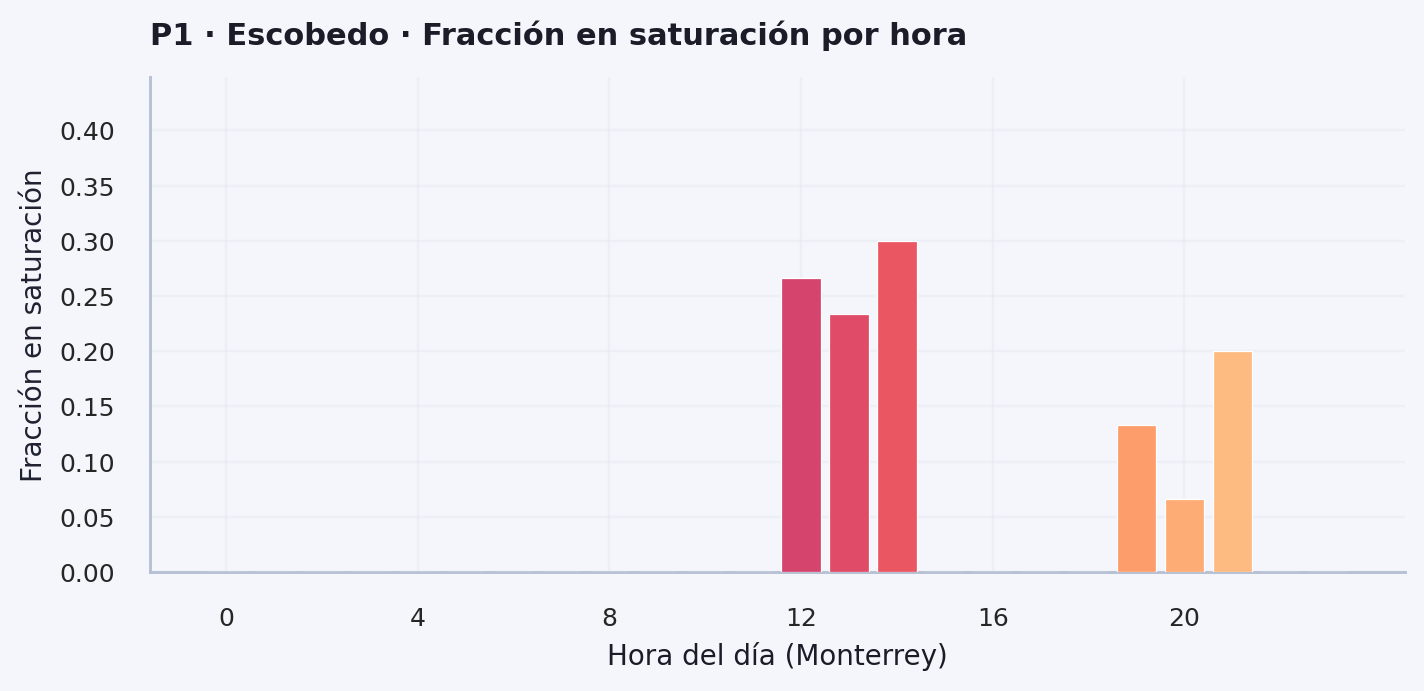
\includegraphics[width=\linewidth,height=0.68\textheight,keepaspectratio]{../modulo1_diagnostico/figures/p1_frecuencia_por_zona/p1_frecuencia_hora__Escobedo.png}
  \par
  \endgroup
  \pizoneread
\end{frame}

\begin{frame}{P1 · Independencia}
  \begingroup
  \centering
  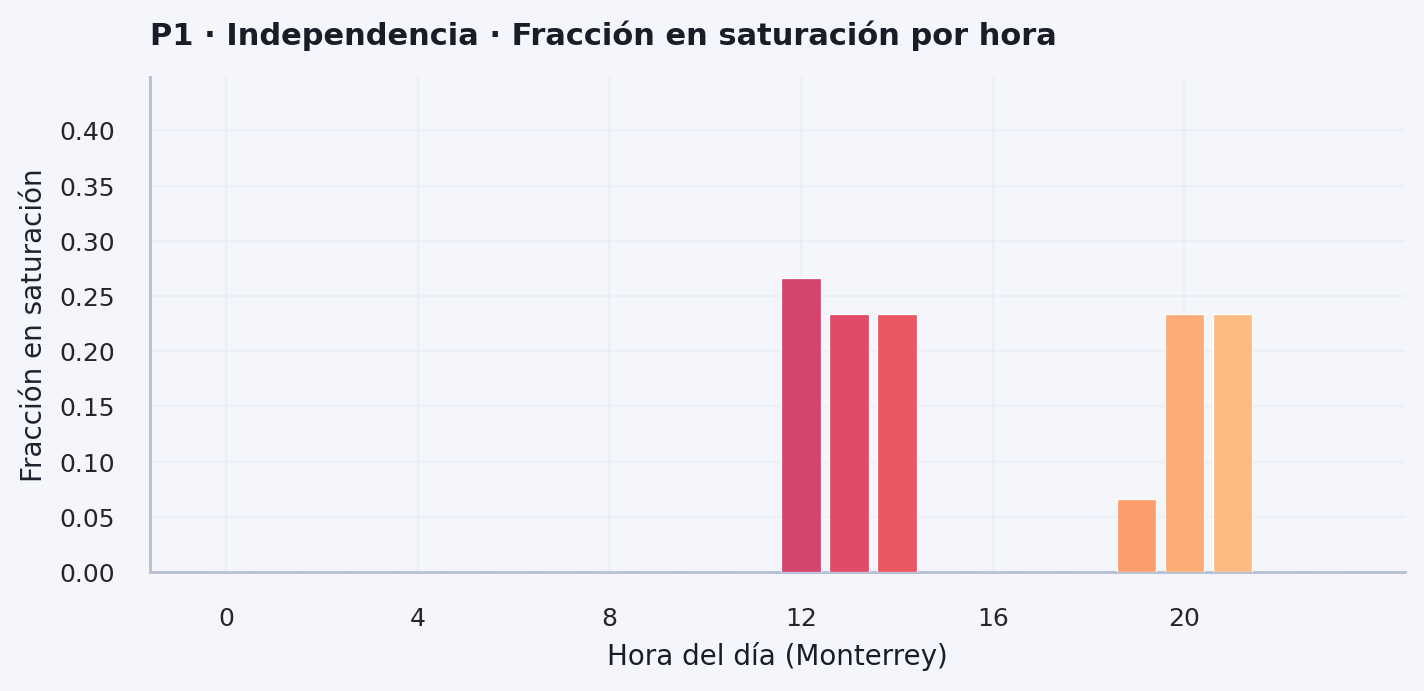
\includegraphics[width=\linewidth,height=0.68\textheight,keepaspectratio]{../modulo1_diagnostico/figures/p1_frecuencia_por_zona/p1_frecuencia_hora__Independencia.png}
  \par
  \endgroup
  \pizoneread
\end{frame}

\begin{frame}{P1 · La Fe}
  \begingroup
  \centering
  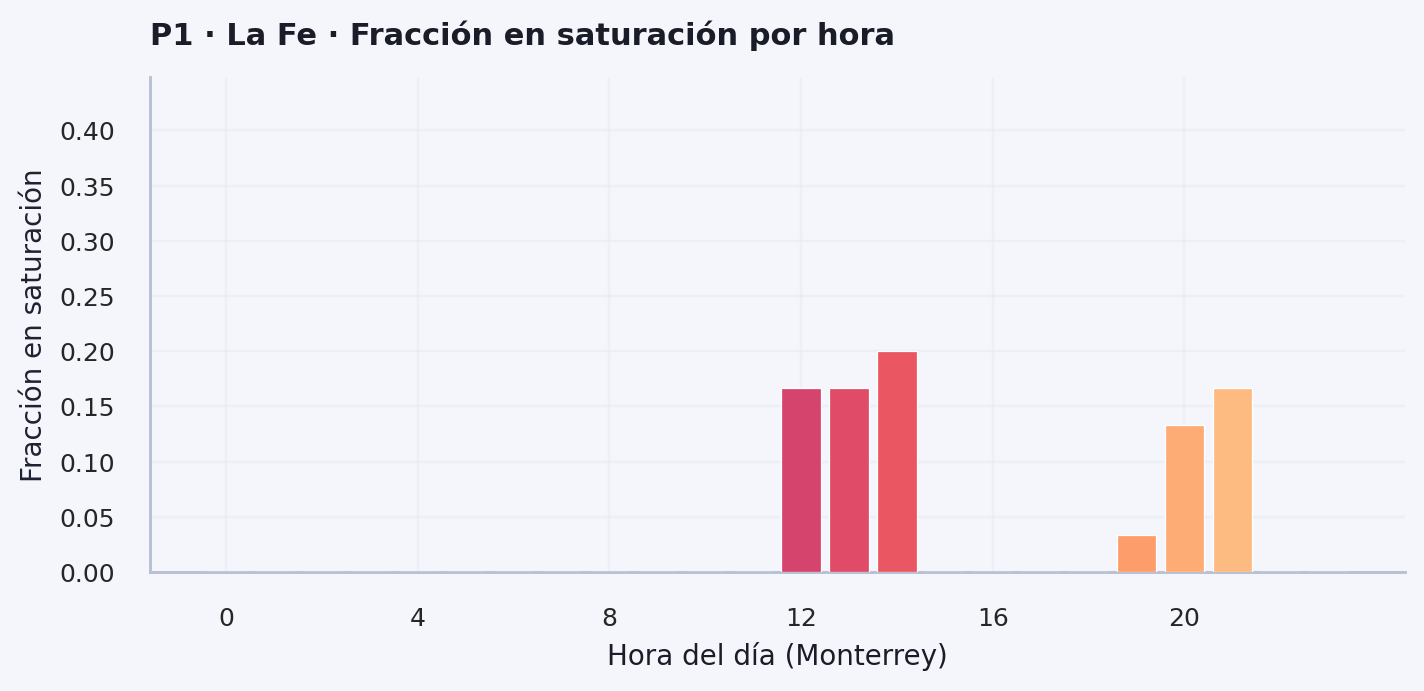
\includegraphics[width=\linewidth,height=0.68\textheight,keepaspectratio]{../modulo1_diagnostico/figures/p1_frecuencia_por_zona/p1_frecuencia_hora__La_Fe.png}
  \par
  \endgroup
  \pizoneread
\end{frame}

\begin{frame}{P1 · Mitras Centro}
  \begingroup
  \centering
  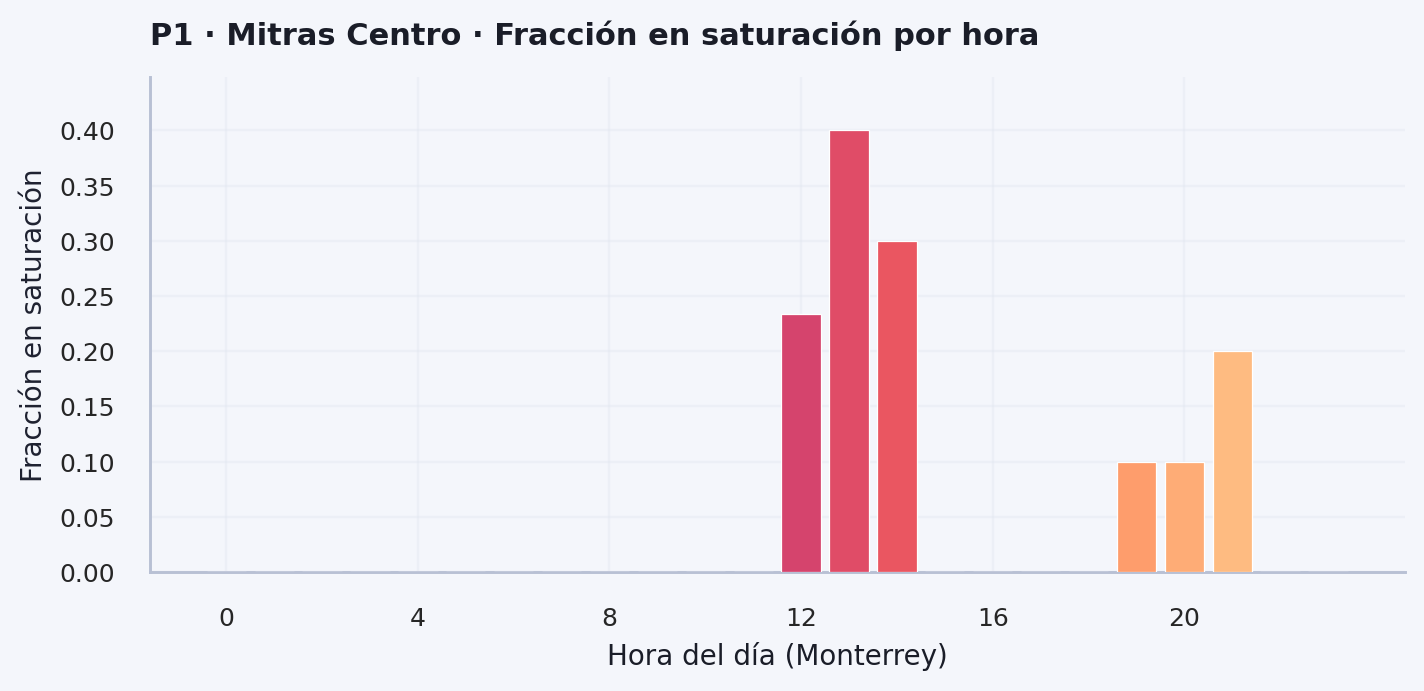
\includegraphics[width=\linewidth,height=0.68\textheight,keepaspectratio]{../modulo1_diagnostico/figures/p1_frecuencia_por_zona/p1_frecuencia_hora__Mitras_Centro.png}
  \par
  \endgroup
  \pizoneread
\end{frame}

\begin{frame}{P1 · MTY Apodaca Huinalá}
  \begingroup
  \centering
  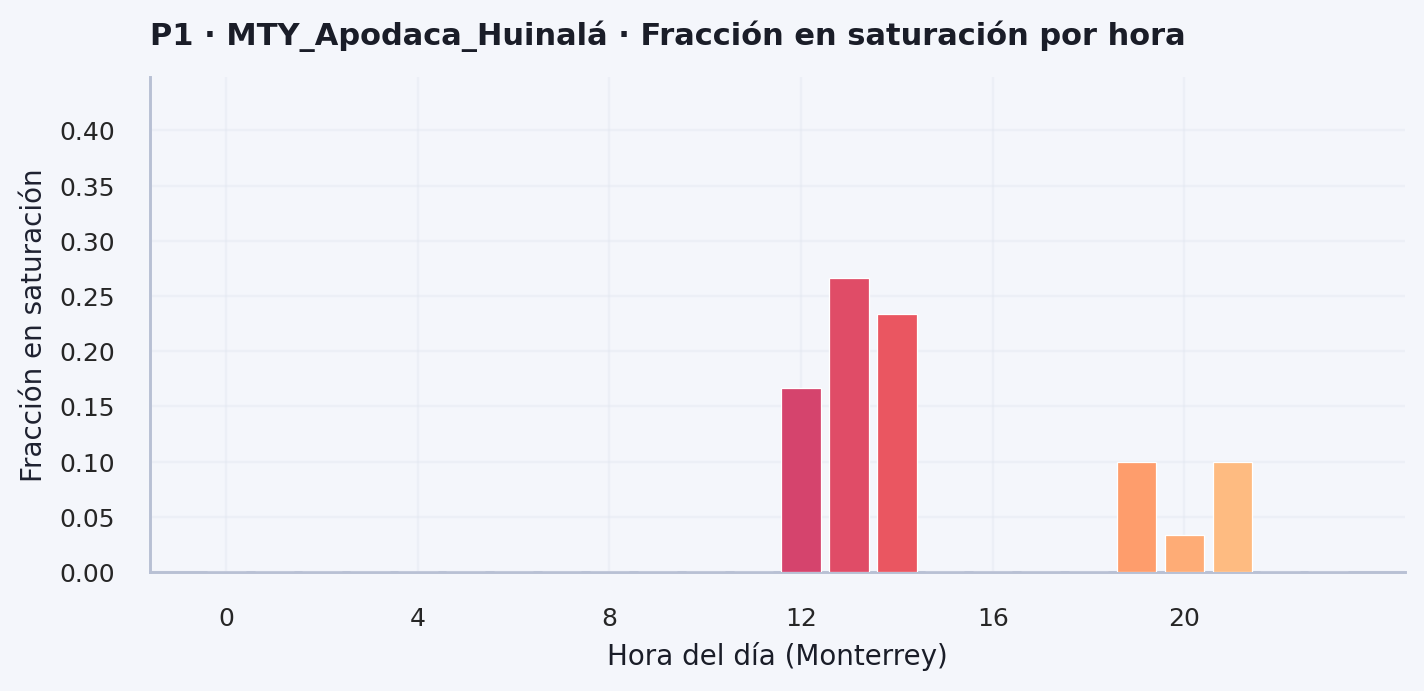
\includegraphics[width=\linewidth,height=0.68\textheight,keepaspectratio]{../modulo1_diagnostico/figures/p1_frecuencia_por_zona/p1_frecuencia_hora__MTY_Apodaca_Huinalá.png}
  \par
  \endgroup
  \pizoneread
\end{frame}

\begin{frame}{P1 · MTY Guadalupe}
  \begingroup
  \centering
  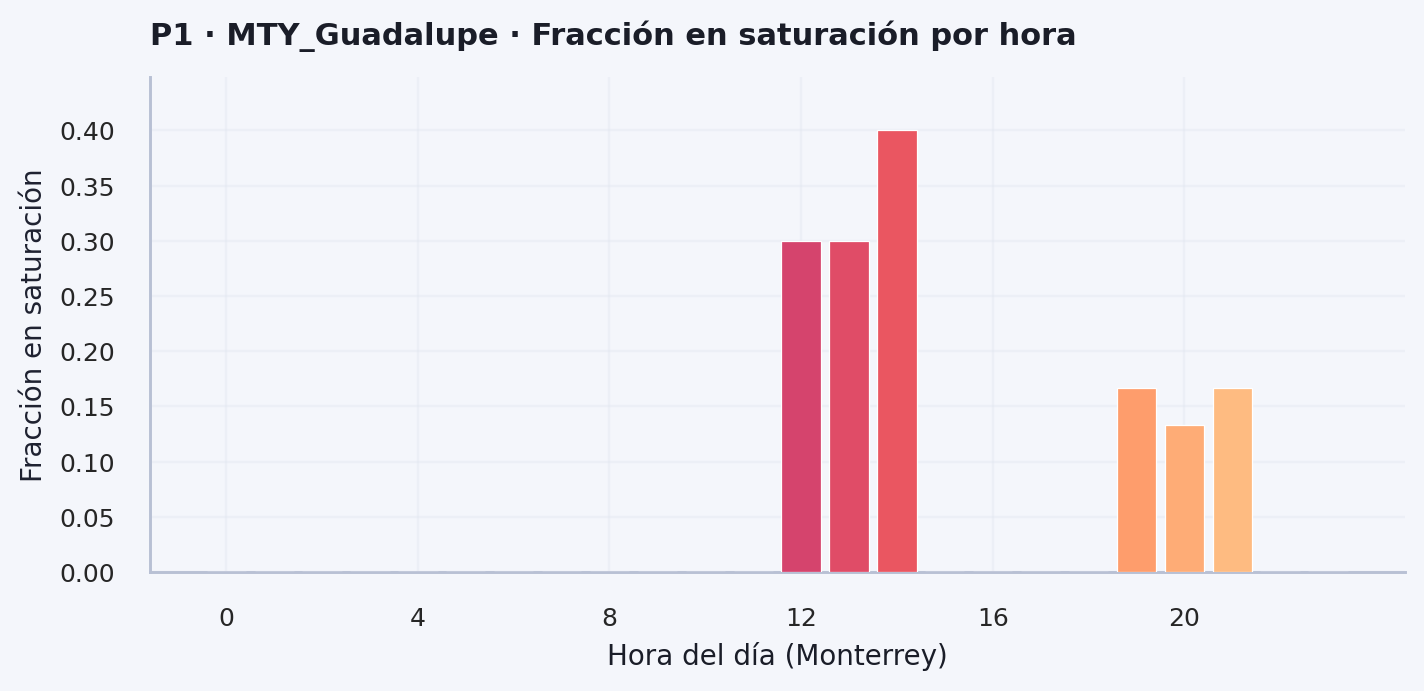
\includegraphics[width=\linewidth,height=0.68\textheight,keepaspectratio]{../modulo1_diagnostico/figures/p1_frecuencia_por_zona/p1_frecuencia_hora__MTY_Guadalupe.png}
  \par
  \endgroup
  \pizoneread
\end{frame}

\begin{frame}{P1 · San Nicolás}
  \begingroup
  \centering
  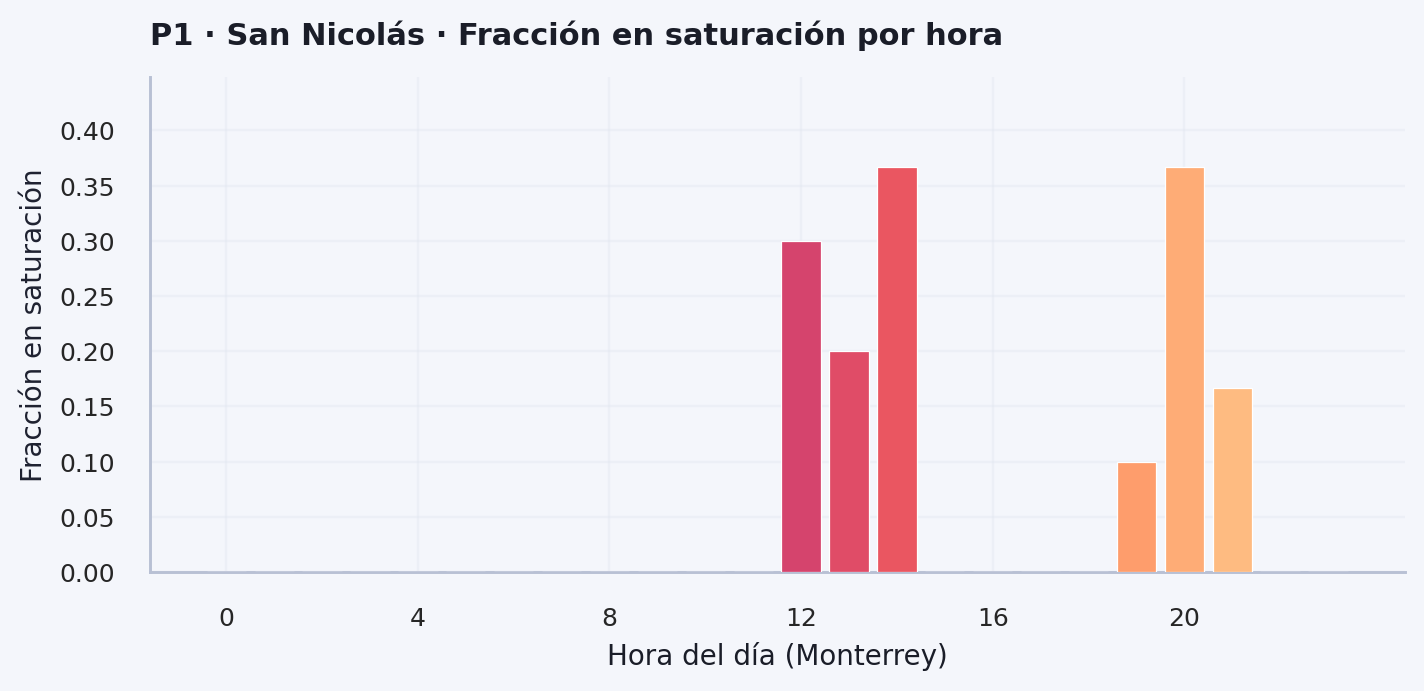
\includegraphics[width=\linewidth,height=0.68\textheight,keepaspectratio]{../modulo1_diagnostico/figures/p1_frecuencia_por_zona/p1_frecuencia_hora__San_Nicolás.png}
  \par
  \endgroup
  \pizoneread
\end{frame}

\begin{frame}{P1 · San Pedro}
  \begingroup
  \centering
  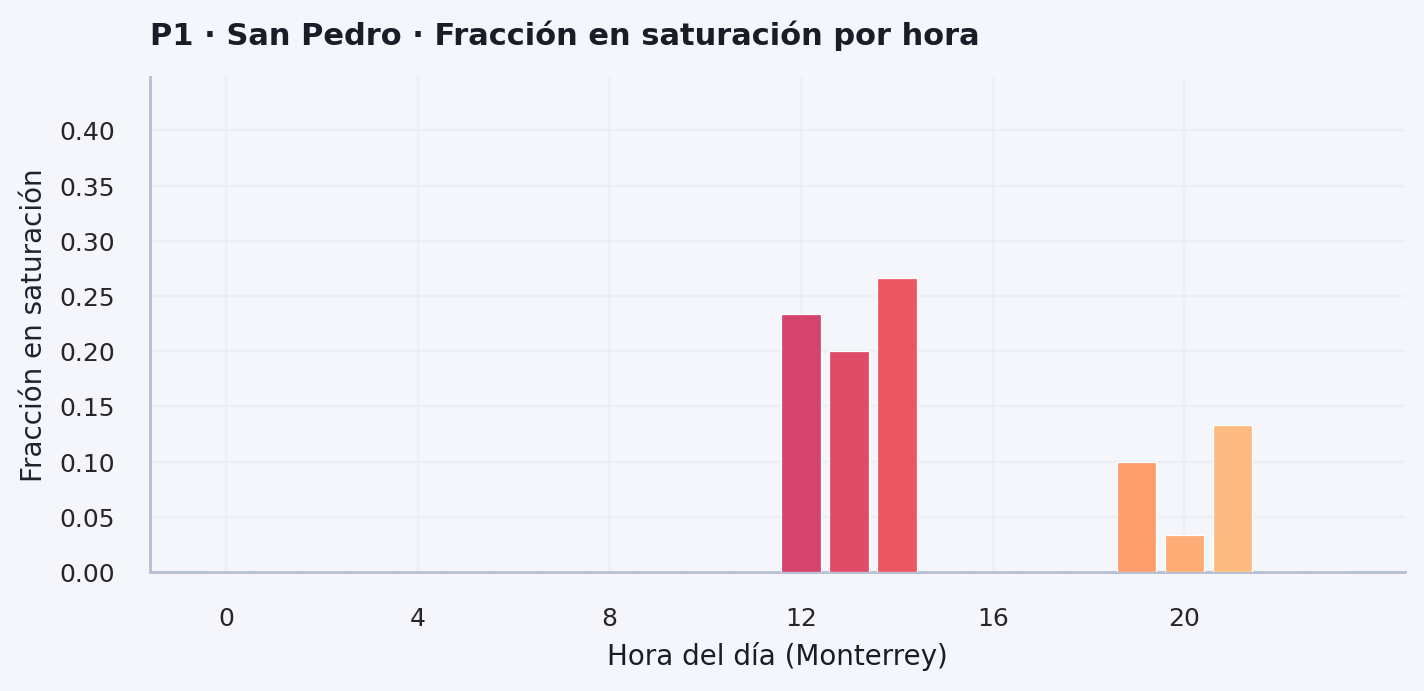
\includegraphics[width=\linewidth,height=0.68\textheight,keepaspectratio]{../modulo1_diagnostico/figures/p1_frecuencia_por_zona/p1_frecuencia_hora__San_Pedro.png}
  \par
  \endgroup
  \pizoneread
\end{frame}

\begin{frame}{P1 · Santa Catarina}
  \begingroup
  \centering
  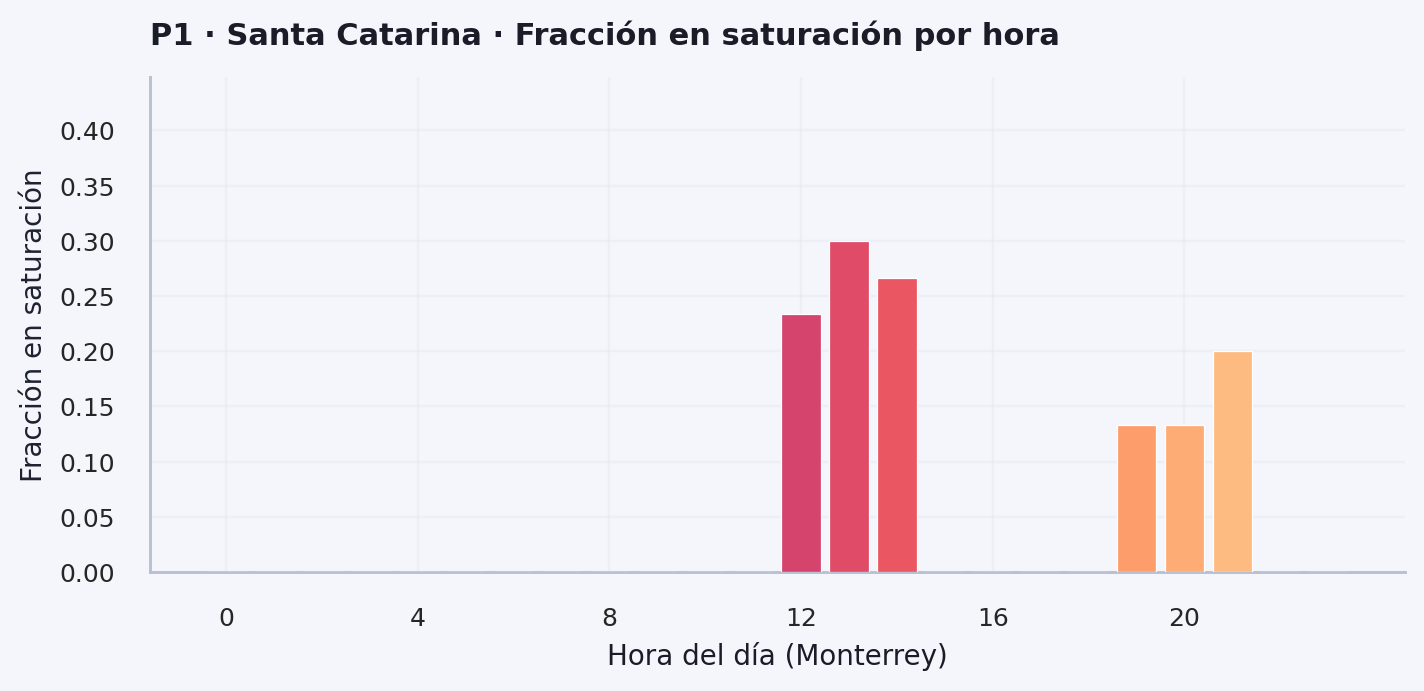
\includegraphics[width=\linewidth,height=0.68\textheight,keepaspectratio]{../modulo1_diagnostico/figures/p1_frecuencia_por_zona/p1_frecuencia_hora__Santa_Catarina.png}
  \par
  \endgroup
  \pizoneread
\end{frame}

\begin{frame}{P1 · Santiago}
  \begingroup
  \centering
  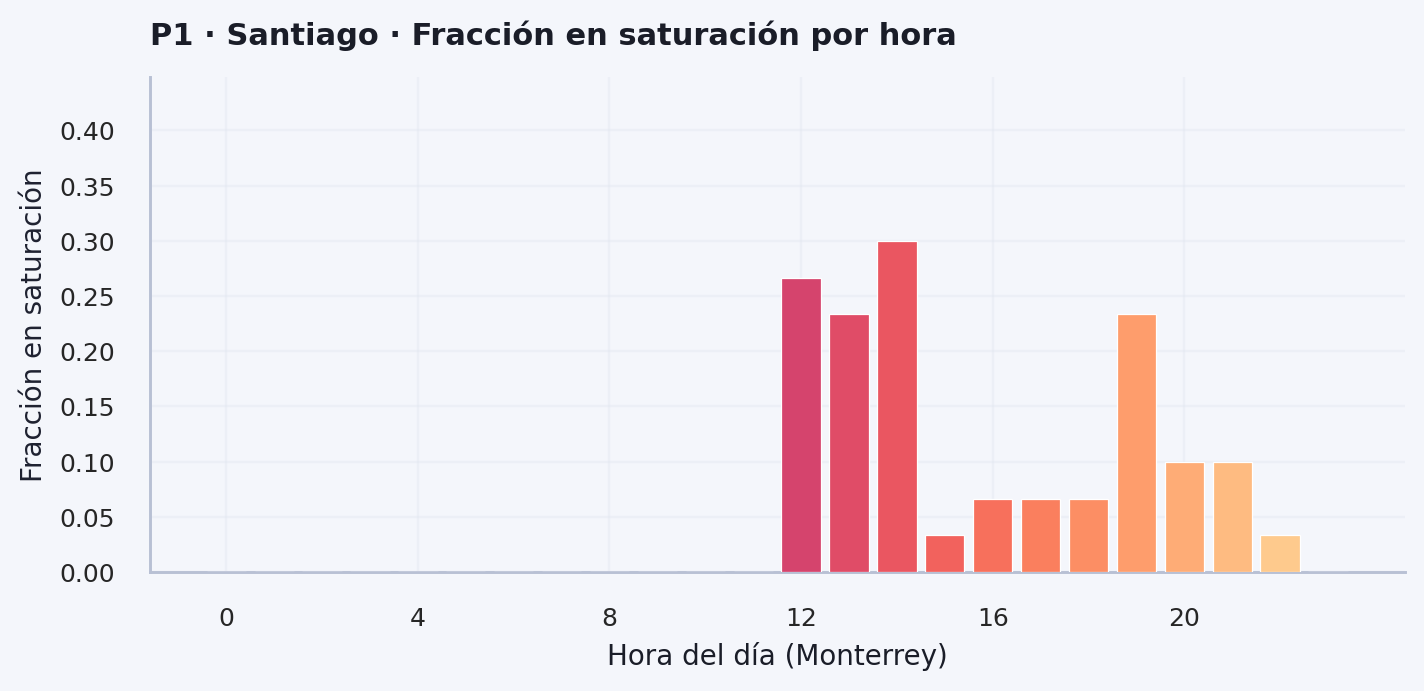
\includegraphics[width=\linewidth,height=0.68\textheight,keepaspectratio]{../modulo1_diagnostico/figures/p1_frecuencia_por_zona/p1_frecuencia_hora__Santiago.png}
  \par
  \endgroup
  \pizoneread
\end{frame}
